\documentclass[main.tex]{subfiles}
\begin{document}
\section{Preliminaries}
\subsection{Free particle (first overview)}
Assume, we want to find a function $\psi: \reals \times \reals \to \C$ which satisfies the following equation:
\begin{equation}
\label{free_particle_equation}
    i\cfrac{\partial \psi(t, x)}{\partial t} = - \cfrac{1}{2m} \cdot \cfrac{\partial^2 \psi(t,x)}{\partial x^2}.
\end{equation}
This happen to be a Schrödinger equation of a free particle in Quantum Mechanics. But we will deal with it purely mathematically and in this subsection we won't need any of Quantum Mechanics.
Very often when the context is clear, we will write $\psi_t(x):=\psi(t,x).$
We need of course to assume that $t\to \psi(t,x)$ is differentiable for all $x\in \reals$ and that $x\to \psi(x, t)$ is two times differentiable for all $t\in \reals$.
If we assume that $\psi_t\in L^1(\reals)$, we can define:
\begin{equation}
    \hat{\psi}(t,p) = \F(\psi_t)(p).
\end{equation}
Then by Theorem \ref{fourier_formal}, the equation (\ref{free_particle_equation}) implies
\begin{equation}
\cfrac{\partial \hat{\psi}(t, p)}{\partial t} = -i \cfrac{p^2}{2m}\cdot \hat{\psi}(t, p).
\end{equation}
The solution for the above equation is given by
\begin{equation}
    \hat{\psi}(t, p) = A(p)\exp(-it\cfrac{p^2}{2m}).
\end{equation}
If we define $\hat{\psi}(p):= \hat{\psi}(0, p)$ then
\begin{equation}
\label{free-momentum-representation}
    \hat{\psi}(t, p) = \hat{\psi}(p)\exp(-it\cfrac{p^2}{2m}).
\end{equation}
If we assume that $\hat{\psi}(p)$ is $L^1(\reals)$ we have a solution of (\ref{free_particle_equation}) $\psi(t, x) = \F^{-1}(\hat{\psi}_t)(x)$ which expands to
\begin{equation}
    \psi(t, x) = \cfrac{1}{\sqrt{2\pi}}\int_{-\infty}^{\infty} \hat{\psi}(p) \exp\big(ip(x - \frac{tp}{2m})\big) dp.
\end{equation}
This is a wave packet.
Note that if $|\hat{\psi}(p)|^2$ is a probability density, then $|\hat{\psi}_t|^2 = |\hat{\psi}(p)|^2$ is a probability density for each $t\in\reals$. Then also Theorem \ref{plancherel} (The Parserval Formula) implies that $|\psi_t|^2$ is a probability density for all $t\in \reals$. We will proceed further under the assumption that $|\hat{\psi}(p)|^2$ is a probability density.
To analyze how the wave packet moves in time it will be useful to introduce some abstract random processes $X_t$ and $P_t$. Let $X_t$ be an arbitrary random process where probability density of $X_t$ is $|\psi_t|^2$ and let $P_t$ be an arbitrary process where probability density of $P_t$ is $|\hat{\psi}_t|^2$. Given that $|\hat{\psi}_t|^2 = |\hat{\psi}(p)|^2$ we will assume $P=P_t$ with probability density $|\hat{\psi}(p)|^2$. We don't assume a joint distribution for $X_t$ and $P_t$, so they can't be read as momentum and position random processes, because in general as Nelson Theorem states: ``The observables $R_1$ and $R_2$ have a joint probability distribution in all states if and only if they commute, that is if and only if $[R_1 , R_2] = 0$.'' (\cite{breure-petruccione2002}, \cite{nelson1967}).
We have
\begin{equation}
    E(X_t) = \int_{-\infty}^{\infty} x\psi(x, t) \overline{\psi(x, t)} dx,
\end{equation}
and 
\begin{equation}
\label{avg_momentum}
    E(P) = \int_{-\infty}^{\infty} p\hat{\psi}(p, t) \overline{\hat{\psi}(p, t)} dp = \int_{-\infty}^{\infty} p\hat{\psi}(p) \overline{\hat{\psi}(p)} dp.
\end{equation}
By Theorem \ref{position_to_momentum}
\begin{equation}
\label{avg_position}
    E(X_t) = \int_{-\infty}^{\infty} i\cfrac{\partial \hat{\psi}}{\partial p}(p,t)\cdot \overline{\hat{\psi}(p, t)} dp.
\end{equation}
Note that
\begin{equation}
    \cfrac{\partial \hat{\psi}}{\partial p}(p, t) = \bigg(\cfrac{d \hat{\psi}}{d p}(p) - \frac{itp}{m} \hat{\psi}(p)\bigg) \exp(-it\cfrac{p^2}{2m}).
\end{equation}
Thus
\begin{equation}
    E(X_t) = \int_{-\infty}^{\infty} i \bigg(\cfrac{d \hat{\psi}}{d p}(p) - \frac{itp}{m} \hat{\psi}(p)\bigg)\overline{\hat{\psi}(p)} dp.
\end{equation}
And from the above, by (\ref{avg_position}) and (\ref{avg_momentum}) we are getting a very nice equation
\begin{equation}
    E(X_t) = E(X_0) + \cfrac{t}{m}E(P).
\end{equation}
Which says that if we consider $t$ as time, the mean value of a random variable with density $|\psi_t|^2$ travels along $x$ axis with a constant velocity $v = \cfrac{\langle P\rangle}{m}$.
Let's now analyze Var($X_t$) to observe $\psi_t$ wave dispersion. Again by Theorem \ref{position_to_momentum}, we have
\begin{equation}
    E(X^2_t) = \int_{-\infty}^{\infty} - \cfrac{\partial^2 \hat{\psi}}{\partial p^2}(p, t) \cdot \overline{\hat{\psi}(p, t)} dp.
\end{equation}
Note that
\begin{equation}
    \cfrac{\partial^2 \hat{\psi}}{\partial p^2}(p, t) = 
    \big(\cfrac{d^2 \hat{\psi}}{d p^2}(p) - 2\cfrac{itp}{m}\cdot\cfrac{d \hat{\psi}}{d p}(p) - \cfrac{it}{m}\hat{\psi}(p) - \cfrac{t^2p^2}{m^2}\hat{\psi}(p)\big)e^{-it\frac{p^2}{2m}}.
\end{equation}
Thus
\begin{equation}
    E(X^2_t) = \int_{-\infty}^{\infty}\bigg(-\cfrac{d^2 \hat{\psi}}{d p^2}(p) + \cfrac{t^2p^2}{m^2}\hat{\psi}(p) + \cfrac{it}{m}\big(2p\cfrac{d \hat{\psi}}{d p}(p) - \hat{\psi}(p)\big)\bigg)\overline{\hat{\psi}(p)} dp.
\end{equation}
Hence
\begin{equation}
    E(X^2_t) = E(X^2_0) + \cfrac{t^2}{m^2}E(P^2) + \int_{-\infty}^{\infty}\cfrac{it}{m}\bigg(2p\cfrac{d \hat{\psi}}{d p}(p) - \hat{\psi}(p)\bigg)\overline{\hat{\psi}(p)} dp,
\end{equation}
and
\begin{equation}
    \text{Var}(X_t) = \text{Var}(X_0) + \cfrac{t^2}{m^2}\text{Var}(P) + 
    \cfrac{t}{m}\bigg(\int_{-\infty}^{\infty}i\big(2p\cfrac{d \hat{\psi}}{d p}(p) - \hat{\psi}(p)\big)\overline{\hat{\psi}(p)} dp - 2E(X_0)E(P)\bigg).
\end{equation}


It is easy to notice that for $\hat{\psi}(p)\in\reals$ for all $p\in\reals$ (it might be helpful to note first that in such case $E(X_0) = 0$.) holds:
\begin{equation}
    \text{Var}(X_t) = \text{Var}(X_0) + \cfrac{t^2}{m^2}\text{Var}(P).
\end{equation}
Note that the reasoning up to this point is purely mathematical, we didn't use any postulates of quantum theory or we didn't use consciously momentum or position operators. However obviously they appeared in calculations. 
Similar but more detailed approach you may find in \cite{hall2013}.
\section{Quantum theory}

\subsection{Naive Momentum and Position Operators}
In this section, unless not stated otherwise, we assume that all $L^p(X)$, $C^n(X)$, $C_0(X)$ etc. are sets of complex valued functions.
We will use symbols $P$ i $Q$ to denote momentum and position operators respectively.
\begin{equation}
    P\psi = -i\cfrac{d}{dx}\psi.
\end{equation}
\begin{equation}
    (Q\psi)(x) = x\psi(x).
\end{equation}
For any two linear operators $A$, $B$ understood at the moment as very abstract linear operations with no explicit domain, we define commutator as $[A, B] = AB - BA$.
\begin{theorem}
Let $\psi:\reals\to\C$ be differntiable function, then
\begin{equation}
\label{[Q,P]}
    [Q, P]\psi = i\psi.
\end{equation}
\end{theorem}
\begin{proof}
\begin{equation}\label{QP}
    QP\psi = Q(-i\frac{d\psi}{dx}) = -ix\frac{d\psi}{dx}.
\end{equation}
\begin{equation}
\label{PQ}
    PQ\psi = P(x\psi) = -i\psi + -ix\frac{d\psi}{dx}.
\end{equation}
If we subtract equation (\ref{PQ}) from equation (\ref{QP}), we got (\ref{[Q,P]}).
\end{proof}
\subsection{Momentum operator in $n$-dimensional space}
Below we will develop in more details what is mentioned in \cite{breure-petruccione2002} (Quantum Probability 2.1) and \cite{hall2013} (Perspectives on the Spectral Theorem 6.6).

In this subsection $\F$ will be a Fourier transform defiend by Definition \ref{extended_fourier}.
The most usual case will be $n=3$, but we also quite often consider particles moving only along the stright line when $n=1$. Mathematically speaking though, we can think even about $n > 3$.

We will define momentum operator, from the perspective of spectral measure. This aproach has following advantages. It is clear from the begining that momentum operator is self-adjoint and there is no problem what is its domain, we don't need to define its domain, we mearly need to discover it. The below definition will be fully understood in the context of Theorem \ref{observable-representation}

\begin{definition}
Let $H=L^2(\reals^n)$. Let $E$ be a spectral measure defined as follows
\begin{equation}
E_{i}(\omega)(\psi) = \F^{-1}(1_{\omega}(x_i)\F(\psi)),
\end{equation}
where $\psi$ is treated as a function of $x=(x_1,\dots, x_n)$.
The momentum operator along the coordinate $i$ is
\begin{equation}
P_i = E_i(\text{id}).
\end{equation}  
\end{definition}
Recall that $\F:L^2(\reals^n)\to L^2(\reals^n)$ is a unitary mapping.
Let's see how much we can derive from the above definition by Theorem \ref{observable-representation}. First we know that $P_i$ is sef-adjoin and that the domain $\mathcal{D}(P_i)$ is dense in $L^2(\reals^n)$. Next, that
\begin{equation}
\mathcal{D}(P_i) = \{\phi \in L^2(\reals^n) : x_i\F(\psi)\in  L^2(\reals^n)\}.
\end{equation} 
and
\begin{equation}
P_i\psi = \F^{-1}(x_i\F(\psi)).
\end{equation}
Which by Theorem \ref{fourier-weak-d} translates imediatelly to
\begin{equation}
\mathcal{D}(P_i) = \{\psi \in L^2(\reals^n) : \mathsf{D}^i\psi\in L^2(\reals^n)\}.
\end{equation}
and
\begin{equation}
P_i\psi = -i\mathsf{D}^i\psi.
\end{equation}
Which for any differentiable $\psi \in L^2(\reals^n)$ means simply
\begin{equation}
P_i\psi = -i\cfrac{\partial \psi}{\partial x_i}.
\end{equation}
Also we see immediately that $\F(\psi)$ is momentum representation of a wave function $\psi$ with
\begin{equation}
\langle  \phi, P_i \psi\rangle = \int x_i \F(\psi)\overline{\F(\phi)} dx^n.
\end{equation}
\begin{example}
Let $\F:L^2(\reals)\to L^2(\reals)$ be the extension of Fourier transform. We will define a spectral measure
\begin{equation}
E(\omega)\psi = \F^{-1}(1_\omega \cdot \F(\psi)).
\end{equation}
Note that for $\psi\in L^2(\reals)\cap L^1(\reals)$ and $\F(\psi)\in L^1(\reals)$.
\begin{equation}
(E(\omega)\psi)(x) = \frac{1}{\sqrt{2\pi}}\int_\omega e^{ixk} \F(\psi)(k)dk.
\end{equation}
$P\psi = E(\text{id})$ is obviously a $1$-dimensional momentum operator.
\end{example}
\section{Harmonic oscillator (first attempt)}
Let's write Schrödinger equation of harmonic oscillator in the following form
\begin{equation}
    i\frac{\partial \psi}{\partial t} = \frac{1}{2m}P^2\psi + \cfrac{1}{2}m\omega^2 Q^2\psi.
\end{equation}
The Hamiltonian in the equation is $H = \frac{1}{2m}P^2 + \cfrac{1}{2}m\omega^2 Q^2$.
We want to find all possible states of energy $E\in \reals$, which are $H$ eigenvalues
\begin{equation}
    H\psi = E\psi.
\end{equation}
for any differentiable $\psi\in L^2(\reals)$. We will put aside domain considerations. All transformation should be true in a Schwartz space $S_1$ (Definition \ref{schwartz-space}) which is dense in $L^2(\reals)$. This statement is not necesarly removing all difficulties, we will perhaps solve this more rigoriously later. At some point it will be good to find proper theorems to deal rigorously with solutions of equations, as for having $P$ self-adjoin we extended domain to weakly differentiable functions -- so now all theorems that say about uniquess of solutions must work for weak deriviatives.
  
Let's define
\begin{equation}
P_0 := \cfrac{1}{\sqrt{2m\omega}}P,
\end{equation}
\begin{equation}
Q_0 := \sqrt{\cfrac{m\omega}{2}}Q.
\end{equation}
Now $H = \omega(P_0^2 + Q_0^2)$.
Note that 
\begin{equation}
[Q_0, P_0] = \cfrac{1}{2}i.
\end{equation}
Thus
\begin{equation}
(Q_0 - iP_0)(Q_0 + iP_0) = Q_0^2 + P_0^2 - \cfrac{1}{2}I.
\end{equation}
Then if we define
\begin{equation}
    A^\dag = Q_0 -iP_0,
\end{equation}
and 
\begin{equation}
    A = Q_0 + iP_0.
\end{equation}
Now, we can write $H$ in the following form
\begin{equation}
    H = \omega(A^\dag A + \frac{1}{2}). 
\end{equation}
Let $N = A^\dag A$.
We will establish first some facts about $A^\dag$ and $A$.

We will write now $A^\dag$ and $A$ explicitly.
\begin{equation}
A^\dag \psi = \sqrt{\cfrac{m\omega}{2}}x\psi - \cfrac{1}{\sqrt{2m\omega}}\cfrac{\partial\psi}{\partial x}.
\end{equation}
\begin{equation}
A \psi = \sqrt{\cfrac{m\omega}{2}}x\psi + \cfrac{1}{\sqrt{2m\omega}}\cfrac{\partial\psi}{\partial x}.
\end{equation}
\begin{fact}
If $\psi \in L^2(\reals)$, $\psi$ is differentiable and  satisfies the equation
\begin{equation}
\label{unique_solution_A}
    A\psi = 0,
\end{equation}
then there exists $C\in \C$ such that
\begin{equation}
    \psi(x) = C\exp(-\frac{m \omega x^2}{2}).
\end{equation}
\end{fact}
\begin{proof}
Equation (\ref{unique_solution_A}) is equivalent to
\begin{equation}
    \cfrac{\partial \psi}{\partial x} = - m\omega x \psi.
\end{equation}
It can be proven that all solutions of the above have a form $\psi(x) = C\exp(-\frac{m\omega x^2}{2})$. Since $\psi\in L^2(\reals)$ it is a valid solution of (\ref{unique_solution_A}).
\end{proof}

\begin{fact}
\label{zero-creator}
    If $\psi\in L(\reals)^2$, $\psi$ is differentiable $A^\dag \psi = 0$, then $\psi=0$.
\end{fact}
\begin{proof}
Here $A\psi = 0$ is equivalent to
\begin{equation}
    \cfrac{\partial \psi}{\partial x} = m\omega x \psi.
\end{equation}
So the solution has a form $\psi(x) = C\exp(\frac{m\omega x^2}{2})$, where $C\in\C$. But we must have $\psi\in L(\reals)^2$, thus the only possible solution is $\psi = 0$.
\end{proof}
Let's now check commutator $[A, A^\dag]$.
\begin{equation}
A^\dag A = Q_0^2 + P_0^2 - \cfrac{1}{2}.
\end{equation}
\begin{equation}
A A^\dag = Q_0^2 + P_0^2 + \cfrac{1}{2}.
\end{equation}
Thus
\begin{equation}
\label{creator-anihilator-commutator}
[A, A^\dag] = 1.
\end{equation}
\begin{fact}
If $\psi, \phi\in S_1$, then
\begin{equation}
\langle A\psi, \phi \rangle = \langle \psi, A^\dag \phi \rangle 
\end{equation}
and
\begin{equation}
\label{N-symmetric}
\langle N\psi, \phi \rangle = \langle \psi, N \phi \rangle.
\end{equation}
\end{fact}
\begin{fact}
If $\gamma$ is an eigenvalue of $N$ with the corresponding eigenvector $\psi\in S_1$,
then $\gamma \geq 0$ and $\gamma + 1$ is an eigenvalue of $N$ with the corresponding eigenvector $A^\dag\psi$.
\end{fact}
\begin{proof}
By (\ref{N-symmetric}), we have $\gamma \geq 0$. By (\ref{creator-anihilator-commutator}) we can calculate the following
\begin{multline}
N A^\dag \psi = A^\dag A A^\dag \psi = A^\dag(1 + A^\dag A)\psi = A^\dag\psi + A^\dag N \psi = A^\dag \psi + \gamma A^\dag \psi = \\
(\gamma + 1) A^\dag \psi. 
\end{multline}
By Fact \ref{zero-creator}, we know that $A^\dag \psi\not = 0$, thus $A^\dag \psi$ is an eigenvector. 
\end{proof}
\begin{fact}
If $\gamma > 0$ is an eigenvalue of $N$ with the corresponding eigenvector $\psi\in S_1$, then $\gamma - 1$ is an eigenvalue of $N$ with the corresponding eigenvector $A\psi$.
\end{fact}
\begin{proof}
By (\ref{creator-anihilator-commutator}), we can calculate the following
\begin{multline}
N A\psi = A^\dag A A \psi = (AA^\dag - 1)A\psi = AN\psi - A\psi = A\gamma\psi - A\psi = (\gamma - 1)A\psi.
\end{multline}
Now we need to show that $A\psi \not= 0$. Indeed, if $A\psi=0$, then $N\psi = 0$, but since $\psi$ is an eigenvector with eigenvalue $\gamma > 0$, this is a contradiction.
\end{proof}
\section{Dirac Formulation of Quantum Mechanics}

\begin{note}
\label{dirac-note}
Note that with Dirac formulation of Quantum Mechanics we operate on spaces wider than Hilbert spaces and sometimes $\bra{\phi_\alpha}\ket{\phi_\beta}$ does not has sense as complex number, but we must see it as distribution coresponding to either $\alpha$ or $\beta$. E.g. if we consider position representation $\bra{x}\ket{y} = \delta(x - y)$.
\end{note}

Bra-ket notation is described in first chapters of \cite{dirac1981}.

\begin{equation}
\bra{\phi}^\dagger := \ket{\phi}, \ket{\phi}^\dagger := \bra{\phi}
\end{equation}

\begin{equation}
\langle\phi| \bigl( c_1|\psi_1\rangle + c_2|\psi_2\rangle \bigr) = c_1\langle\phi|\psi_1\rangle + c_2\langle\phi|\psi_2\rangle \,,
\end{equation}



\begin{equation}
\bigl(c_1|\psi_1\rangle + c_2|\psi_2\rangle\bigr)^\dagger = c_1^* \langle\psi_1| + c_2^* \langle\psi_2| \,,
\end{equation}

\begin{equation}
\{\bra{\phi}A\}\ket{\psi} = \bra{\phi}\{A\ket{\psi}\},
\end{equation}

\begin{equation}
A^\dagger \ket{\phi}:= \{\bra{\phi}A\}^\dagger,
\end{equation}

\begin{equation}
\bra{\phi} A^\dagger:= \{A\ket{\phi}\}^\dagger.
\end{equation}

\subsection{Observables}

\begin{definition}
A non zero quantum state $\ket{\phi}$ is called a ket related eigenstate of an linear operator $A$ belonging to the ket related eigenvalue $a \in R$ iff $A\ket{\phi} = a\ket{\phi}$.
\end{definition}

\begin{definition}
A non zero quantum state $\ket{\phi}$ is called a bra related eigenstate of an linear operator $A$ belonging to the bra related eigenvalue $a \in R$ iff $\bra{\phi}A = a\bra{\phi}$.
\end{definition}

In \cite{dirac1981}, Dirac defines \textit{real linear operator} as self-adjoint (i.e. $A^\dagger = A$). The name is justified for a few reasons. The condition $A^\dagger = A$ is analogous for $a^* = a$ for numbers. But also, what we will prove next, \textit{real linear operators} have real eigenvalues.

\begin{proposition}
Let $A$ be a real linear operator and $\ket{\phi}$ be a non-zero quantum state. The following holds:
\begin{equation}
A\ket{\phi} = a\ket{\phi} \implies a\in\R,
\end{equation}

\begin{equation}
\bra{\phi} A = a\bra{\phi} \implies a\in\R,
\end{equation}

\begin{equation}
A\ket{\phi} = a\ket{\phi} \text{ and } \bra{\phi} A = b\bra{\phi} \implies a = b.
\end{equation}

\end{proposition}
\begin{proof}
Since $A = A^\dagger$, we have
\begin{equation}
a\bra{\phi}\ket{\phi} = \bra{\phi} a \ket{\phi} = \bra{\phi} A \ket{\phi} = \bra{\phi} A^\dagger \ket{\phi} = \bra{\phi} a^* \ket{\phi} = a^* \bra{\phi}\ket{\phi}.
\end{equation}
Also
\begin{equation}
a\bra{\phi}\ket{\phi} = \bra{\phi} a \ket{\phi} = \bra{\phi} A \ket{\phi} = \bra{\phi} b \ket{\phi} = a\bra{\phi}\ket{\phi},
\end{equation}
thus $a = b$.
\end{proof}

The above results justifies, that for real linear operators we speak only about eigenstates and eigenvalues not bothering with distinguishing ket and bra kinds.

\begin{proposition}
\label{orthogonal-fact}
Let $A$ be a real linear operator. If two eigenstates $\ket{\phi}, \ket{\psi}$ belong to different eigenvalues, then $\bra{\phi}\ket{\psi} = 0$.
\end{proposition}
\begin{proof}
Assume that eigenvalues for $\ket{\phi}, \ket{\psi}$ are correspondingly $a_\phi$ and $a_\psi$. Note that
\begin{equation}
\bra{\phi}A\ket{\psi} = \bra{\phi}a_\psi\ket{\psi} = \bra{\phi}a_\phi\ket{\psi},
\end{equation}
thus
\begin{equation}
(a_\psi - a_\phi) \bra{\phi}\ket{\psi} = 0.
\end{equation}
And since $a_\psi \not= a_\phi$, we have $\bra{\phi}\ket{\psi} = 0$.
\end{proof} 

\begin{definition}
Let $A$ be a real linear operator.
$\mathcal{E}_A(a)$ denotes a subspace of all eigenstates which belongs to the eigenvalue $a$.
\end{definition}

Note that if $A$ is a real linear operator, then $\mathcal{E}_A(a_1) \perp \mathcal{E}_A(a_1)$ for $a_1 \not= a_2$.

\begin{definition}
A real linear opeartor $A$ acting on a space of quantum states is an observable iff there exists a basis consisted of eigenstates of $A$.  
\end{definition}

Form \ref{orthogonal-fact} it follows that we can always orthogonalise such basis. Indeed, eigenstates which belongs to different eigenvalues are already orthogonal. All eigenstates belonging to one eigenvalue form a subspace of quantum states, so we can take all orthogonals bases from these subspaces and they will form orthogonal bases of the whole quantum state space.

Also the converse holds, if we can find orthogonal base of eigenstates belonging to real eigenvalues, the linear operator is an observable. Let's formulate this in the following proposition.

\begin{proposition} If $A$ is a linear opeartor whose all eigenstates belong to real eigenvalues and form an orthogonal basis, then $A = A^\dagger$ (thus $A$ is an observable). 
\end{proposition}
\begin{proof}
Without loss of genarlity, we can assume that $\ket{\alpha}$ is an orthonormal basis which consits of eigenstates of $A$ such that $A \ket{\alpha} = a(\alpha)\ket{\alpha}$. Take any quantum state $\ket{\phi}$ and express it in the basis $\ket{\alpha}$
\begin{equation}
\ket{\phi} = \int \bra{\alpha}\ket{\phi}\ket{\alpha} d\alpha.
\end{equation}
Note that 
\begin{equation}
A\ket{\phi} = \int a(\alpha) \bra{\alpha}\ket{\phi}\ket{\alpha} d\alpha.
\end{equation}
From the above follows
\begin{equation}
\bra{\psi}(A\ket{\phi}) = \int a(\alpha) \bra{\alpha}\ket{\phi}\bra{\psi}\ket{\alpha} d\alpha.
\end{equation}
for an arbitrary two quantum states $\ket{\phi}, \ket{\psi}$.
Now, 
\begin{multline*}
\\
(\bra{\phi}A^\dagger)\ket{\psi} = \bra{\psi}(A\ket{\phi})^* = \int a(\alpha)^* \bra{\phi}\ket{\alpha}\bra{\alpha}\ket{\psi} = \\ 
\int a(\alpha) \bra{\alpha}\ket{\psi} \bra{\phi}\ket{\alpha} = \bra{\phi}(A\ket{\psi}).\\
\end{multline*}
Because the above equality holds for an arbitrary two quantum states $\ket{\phi}, \ket{\psi}$, we have $A = A^\dagger$.
\end{proof}



\begin{proposition}
\label{eigenstate-representation}
Let $A$ be an observable. If $\ket{a, x}$ is an orthonormal basis, such that $\ket{a, x}$ is an eigenstate belonging to the eigenvalue $a$ (we use $x$ to denote that there might be more than one eigenstates for eigenvalue $a$), then any eigenstate which belongs to eigenvalue $a$ can be represented as
\begin{equation}
\ket{\phi} = \int \bra{a, x}\ket{\phi} \ket{a, x} d x.
\end{equation}
\end{proposition}
\begin{proof}
This becomes obvious if we remeber that eigenstates of different eigenvalues are orthogonal.
\end{proof}
\subsection{Commuting observables}

Let's recall
\begin{equation}
[A, B] = AB - BA.
\end{equation}

Blow theorem is not strict in mathematical sense.

\begin{definition}
Two observables $A, B$ commute iff $[A, B] = 0$.
\end{definition}

The theorem below is not a theorem in a stric mathematical sense. In the light of Note \ref{dirac-note}, we need to require from it some additional compatibility of observables, which means at least that each needs to be well defined on the other's base.

\begin{theorem}
If $A, B$ are commuting observables then there exists an orthogonal base of common eigenstates.
\end{theorem}
\begin{proof}
Assume that $\ket{b,x}$ is an orthonormal basis such that $B \ket{b,x} = b \ket{b,x}$.
Firstly, we will show that $A \ket{b,x} \in \mathcal{E}_B(b)$. Indeed,
\begin{equation}
B(A \ket{b,x}) = A(B \ket{b,x}) = A(b \ket{b,x}) = b A\ket{b,x}.
\end{equation}
Thus by Proposition \ref{eigenstate-representation}, we have 
\begin{equation}
\label{eigen-limitation}
A \ket{b,x} = \int \bra{b, x'} A \ket{b, x} \ket{b, x'} d x'.
\end{equation}
Let $\ket{\phi}$ be an arbitrary eigenstate of $A$. Thus we have ceratin $a\in \R$ such that 
$A \ket{\phi} = a \ket{\phi}$. Let's express $\ket{\phi}$ in basis $\ket{b,x}$:
\begin{equation}
\ket{\phi} = \int \phi_{b, x} \ket{b,x} db dx,
\end{equation}
where $\phi_{b, x}$ are some complex coefficients for which the equation holds.
Because $\ket{\phi}$ is an eigenstate of $A$ belonging to eigenvalue $a$ we have:
\begin{equation}
\int \phi_{b, x} \big( A\ket{b, x} - a\ket{b, x}\big)dbdx = 0.
\end{equation}


Let's substitute $A\ket{b, x}$ using equation (\ref{eigen-limitation}) and expand $\ket{b, x}$ in the bases of subspace of all eigenstates of $B$ with eigenvalue $b$.

\begin{equation}
\int \phi_{b, x} \bigg( \int \bra{b, x'} A \ket{b, x}  \ket{b, x'} d x' - a\int \bra{b, x'}\ket{b, x}  \ket{b, x'} d x'\bigg)dbdx = 0.
\end{equation}
\begin{equation}
\int \phi_{b, x} \bra{b, x'} A - a \ket{b, x}  \ket{b, x'}  d x'dbdx = 0.
\end{equation}

\begin{equation}
\int \bigg(\int \phi_{b, x} \bra{b, x'} A - a \ket{b, x}dx\bigg)  \ket{b, x'} d x' db = 0.
\end{equation}

\begin{equation}
\int \bra{b, x'} (A - a)P_b \ket{\phi} \ket{b, x'} d x' db = 0,
\end{equation}

where $P_b$ is a projection into subspace $\mathcal{E}_B(b)$ (i.e.  $\ket{\phi} = \int \phi_{b, x} \ket{b, x}dx$.)

Thus for any eigenvalue $b$ we have $\bra{b, x'} (A - a)P_b \ket{\phi} = 0$ for each $x'$ and therefore $(A - a)P_b \ket{\phi} = 0$. Thus $P_b \ket{\phi}\in \mathcal{E}_A(a)$.
Since $\ket{\phi}$ was an arbitrary eigenstate of $\mathcal{E}_A(a)$, we showed that
\begin{equation}
P_b \mathcal{E}_A(a) \subset \mathcal{E}_A(a). 
\end{equation} 

Note that since $\mathcal{E}_A(a)$ for all eigenvalues $a$ span entire quantum state space, $P_b \mathcal{E}_A(a)$ for all eigenvalues $a$ span $\mathcal{E}_B(b)$ subspace. But this means that we can find an orthonormal base $\ket{a,u}$ of $\mathcal{E}_B(b)$ such that $A \ket{a,u} = a \ket{a,u}$ and obviously $B \ket{a,u} = b \ket{a,u}$. And sice $\mathcal{E}_B(b)$ for all eigenvalues $b$ span entire quantum space, this proves the thesis.

\end{proof}

The above theorem extends to: 

\begin{theorem}
If $A_1, \dots, A_n$ are commuting observables then there exists an orthogonal base of common eigenstates.
\end{theorem}
  
\subsection{Some properties of Dirac $\delta$}
\label{dirac-delta-basic}
\begin{fact}
\begin{equation}
\\
(2\pi)^{n}\delta(k) = \int_{\R^n} e^{ikx}dx\\
\end{equation}
\end{fact}
\begin{proof}
Let's calculate now Fourier Transform of Dirac delta:
\begin{multline}
\F(\delta_0)(\phi) = \delta_0 (\F(\phi)) = \F(\phi)(0) =  \int_{\R^n} \phi(x) e^{-ix\cdot 0}dx = \\
(2\pi)^{-\frac{n}{2}} \int_{\R^n} \phi(x) \cdot 1 dx =  (2\pi)^{-\frac{n}{2}} 1(\phi).
\\
\end{multline}
Thus
\begin{equation}
\F(\delta_0) = (2\pi)^{-\frac{n}{2}} \cdot 1,
\end{equation}
and 
\begin{equation}
\delta_0 = (2\pi)^{-\frac{n}{2}} \cdot \F^{-1}(1).
\end{equation}
The thesis holds in distrubutions sense.
\end{proof}
\begin{fact}
\begin{equation}
\label{sin2-delta}
\lim_{n\to \infty} \cfrac{\sin^2(nx)}{\pi nx^2} = \delta(x).
\end{equation}
\end{fact}
\begin{proof}
It is known that
\begin{equation}
\int_{-\infty}^{\infty}\cfrac{\sin^2(z)}{z^2}dz = \pi.
\end{equation}
By substitution $z = nx$, $dz = ndx$ we will get thesis.
\end{proof}

\begin{lemma}
\begin{equation}
\cfrac{e^{itE} - 1}{E}\cdot \cfrac{e^{-itE} - 1}{E} = \cfrac{\sin^2(\frac{tE}{2})}{(\frac{E}{2})^2}.
\end{equation}
\end{lemma}
\begin{proof}
\begin{multline*}\\
\cfrac{1 - e^{itE}}{E}\cdot \cfrac{1 - e^{-itE}}{E} = \cfrac{2 - e^{itE} - e^{-itE}}{E^2}
= \cfrac{2(1 - \cos(tE))}{E^2} = 4 \cfrac{\sin^2(\frac{tE}{2})}{E^2}.
\end{multline*}
\end{proof}

\begin{corollary}
\begin{equation}
\lim_{t\to\infty} \cfrac{1}{t} \cdot  \cfrac{1 - e^{itE}}{E}\cdot \cfrac{1 - e^{-itE}}{E} = \delta(E).
\end{equation}
\end{corollary}

\begin{fact}
\begin{equation}
\lim_{\epsilon\to 0} \cfrac{1}{\pi}\cfrac{\epsilon}{x^2 + \epsilon^2} = \delta(x),
\end{equation}

\end{fact}
\begin{proof}
Recall that
\begin{equation}
\cfrac{d}{dz}\arctan(z) = \cfrac{1}{1 + z^2},
\end{equation}
thus
\begin{equation}
\int_{-\infty}^\infty \cfrac{1}{1 + z^2} dz = \pi.
\end{equation}

By substitution $x = \epsilon z$, we have

\begin{equation}
\int_{-\infty}^\infty \cfrac{1}{1 + (\frac{z}{\epsilon})^2} \cfrac{1}{\epsilon} dx = \pi,
\end{equation}

which results in 

\begin{equation}
\int_{-\infty}^\infty \cfrac{\epsilon}{\epsilon^2 + x^2} dx = \pi,
\end{equation}
which proves thesis.

\end{proof}

\begin{fact}
\label{delta-zeros}
If $\delta$ is Dirac delta and $x\in \R^n$, then
\begin{equation}
\delta(f(x)) = \sum_i \cfrac{1}{|\det (\nabla f)(x_i)|}\delta(x-x_i),
\end{equation}

where $x_i$ are all discrete zeros of a real function $f$.
\end{fact}

\begin{proof}
Let $y$ depends on $z$ in a following way $y = f(z)$.
\begin{multline*}
\\
\delta(f(x)) = \int \delta(f(z))\delta(z - x) dz = \sum_i \int\limits_{O_\epsilon(x_i)}
\delta(f(z))\delta(z - x) dz \\
= \sum_i \int\limits_{f(O_\epsilon(x_i))}
\delta(y)\delta(z - x) |\det \frac{\partial z}{\partial y}| dy = \sum_i \int\limits_{f(O_\epsilon(x_i))}
\delta(y)\delta(z - x) |\cfrac{1}{\det \frac{\partial y}{\partial z}}| dy
\\ =   \sum_i \cfrac{1}{|\det (\nabla f)(x_i)|}\delta(x_i-x),
\\
\end{multline*}
where the last equality holds because on a $f(O_\epsilon(x_i))$ variable $z$ is a function of $y$ and for $y=0$ we have $z = x_i$. 
\end{proof}

\begin{corollary}
If $\delta$ is Dirac delta and $x\in \R$, then
\begin{equation}
\delta(f(x)) = \sum_i \cfrac{1}{|f'(x_i)|}\delta(x-x_i),
\end{equation}
where $x_i$ are all discrete zeros of a real function $f$.
\end{corollary}

\subsection{Representations}

Short and incomplete digest from \cite{dirac1981}[III. Representations]

We will use all the time symbol $\delta$ but it depends on measure if it is Dirac delta or Kronecker delta.  
Let $\ket{\alpha}$ be states of orthogonal basis normed in the following way $\bra{\alpha}\ket{\beta} = 0$ for $\alpha \not=\beta$ and $\int \bra{\alpha}\ket{\beta} d\alpha = 1$.
\begin{definition}
Let $A_1, \dots, A_k$ be set of commuting observables and $f$ is a real valued function. Then we define observable
\begin{equation}
f(A_1, \dots, A_k)\ket{\alpha} = f(\lambda_1, \dots, \lambda_n)\ket{\alpha},
\end{equation}
where $A_i \ket{\alpha} = \lambda_i \ket{\alpha}$.  
\end{definition}

\begin{definition}
Commuting observables $A_1, \dots, A_k$ are called independent, if and only if for any observable 
$A_i$ there is no real function $f$ such that $A_i = f(A_1, \cdots, A_{i-1}, A_{i+1}, \cdots A_k)$.
\end{definition}

\begin{definition}
Commuting observables $A_1, \dots, A_k$ are called complete, if for any observable $B$ with the same eigenstates basis 
\begin{equation}
B = f(A_1,  \dots, A_k).
\end{equation}
\end{definition}

\begin{fact}
If $A_1, \dots, A_n$ are commuting and complete observables then base states can be uniquely represented as 
\begin{equation}
\ket{\alpha} = \ket{\lambda_1, \dots, \lambda_n},
\end{equation}
where $A_i \ket{\alpha} = \lambda_i \ket{\alpha}$.  
\end{fact}
\begin{proof}
Assume to the contrary that we have the whole subspace of states $\ket{\beta}$ such that $A_i \ket{\beta} = \lambda'_i \ket{\beta}$ for fixed $\lambda'_i$. Then the basis state $\ket{\alpha}$ will be represented as
\begin{equation}
 \ket{\alpha} = \ket{\lambda_1, \dots, \lambda_n, \theta_1, \dots, \theta_k}.
\end{equation}
Let's define $L_i\ket{\alpha} = \theta_i \ket{\alpha}$. But because $A_1, \dots, A_n$ are complete $L_i = f_i(A_1, \dots, A_n)$ and thus $\theta_i = f_i(\lambda_1, \cdots, \lambda_n)$. Therefore unique set of  $\lambda_1, \dots, \lambda_n$ defines unique basis vector $\ket{\alpha}$.
\end{proof}

The above representation can be normalised in the following way
\begin{equation}
\bra{\lambda'_1, \dots, \lambda'_n}\ket{\lambda_1, \dots, \lambda_n} = \delta(\lambda'_1 - \lambda_1)\dots\delta(\lambda'_n - \lambda_n).
\end{equation}

\subsection{Unitary transformations}
\label{unitary-transformations}
Assume $\ket{\alpha}$ is a normalised basis where $\alpha$ is a vector of eigenvalues for the system of complete commuting observables. Two different basis states $\ket{\alpha}$ and $\ket{\beta}$ must be orthogonal, because at least one eigenvalue needs to be different. We will additionally assume they are normalised $\bra{\alpha}\ket{\beta}= \delta(\alpha - \beta)$. 

Assume we have an isometry $u$ on a space of these vectors. Then 

Consider transformation of quantum states
\begin{equation}
U \ket{\alpha} = \ket{u(\alpha)}.
\end{equation} 

Because $U$ transforms basis states to basis states it can be extended to linear operator on the whole states space.

We will show that $U$ is unitary (i.e. $U^\dag U = U^\dag U = I$.)

\begin{multline*}
\\
\bra{\beta}U^\dag U \ket{\alpha} = \bra{u(\beta)}\ket{u(\alpha)} = \delta(u(\beta) - u(\alpha)) = 
\delta(\beta - \alpha) = \bra{\beta}\ket{\alpha}.\\
\end{multline*} 

The equality $\delta(u(\alpha) - u(\beta)) = \delta(\alpha - \beta)$ holds because $u$ is an isometry (i.e. $|\det (\nabla u)| = 1$) and by Fact \ref{delta-zeros}.

In general case where $u$ is just an arbitrary $1-1$ and "onto" map from the representation space of all eigenvalues vectors for the system of complete observables into the other representation space of all eigenvalues of vectors for the system of complete observables (we don't even require the kets will be from the same states space) the transformation given by
\begin{equation}
U \ket{\alpha} = |\det (\nabla u(\alpha))|^{1/2} \ket{u(\alpha)}
\end{equation} 
is unitary provided both $\ket{\alpha}$ and $\ket{u(\alpha)}$ are normalised.

The other fact which is worth to note is that if we transform space of states with an arbitrary unitary transformation $U$ as
\begin{equation}
\ket{\alpha} \mapsto U\ket{\alpha},
\end{equation} 

then any linear operator $A$ transforms in a way
\begin{equation}
A \mapsto UAU^\dag.
\end{equation}

Indeed, it is enough to notice
\begin{equation}
\bra{\beta}U^\dag(UAU^\dag)U \ket{\alpha} = \bra{\beta} A \ket{\alpha}.
\end{equation}



\subsection{Momentum and Position}

Let us consider states of one non-relativistic particle for which we assume that can be fully described as superpositions of locations in $R^3$. By $\ket{x}$ we will denote a quantum state which describe a particle being ``around" point $x\in \R^3$. We understand ``around" in Dirac delta sense
\begin{equation}
\bra{x_1}\ket{x_2} = \delta(x_2 - x_1).
\end{equation}

Dirac delta provides nice normalisation where
\begin{equation}
\int \ket{x}\bra{x}\ket{z}dx = \int \ket{x}\delta(z - x) dz = \ket{z},  
\end{equation}    

as expected.

Similarity by $\ket{p}$ we denote a quantum state, which describes a quantum state of particle which has a momentum ``around" $p\in \R^3$ (as you can notice usage of letter $p$ is important for this convention, because only by usage of the letter we distinguish this from position representation).

Now, it seems to be a law of the nature that canonical momentum operator is defined as follows
\begin{equation}
\bra{x}P_k\ket{\phi} = -i\hbar \cfrac{\partial}{\partial x^k} \bra{x}P_k\ket{\phi},
\end{equation}

where $x=[x^1, x^2, x^3]$. Consider $\bra{x}P\ket{p}$ resolving it once from bra once from ket side. This leads to the following partial derivatives equations:
\begin{equation}
p^k \bra{x}\ket{p} = -i\hbar \cfrac{\partial}{\partial x^k} \bra{x} \ket{p},
\end{equation}
where $p = [p^1, p^2, p^3]$.

This leads to the following solution

\begin{equation}
\boxed{
\bra{x}\ket{p} = (2\pi\hbar)^{-\frac{3}{2}} \exp(i\cfrac{p\cdot x}{\hbar})
}
\end{equation}

$(2\pi\hbar)^{-\frac{3}{2}}$ is a normalisation constant required by

\begin{equation}
\bra{p_1}\ket{p_2} = \delta(p_2 - p_1).
\end{equation} 

Indeed, first note that (as proved for for (\ref{dirac-delta-as-one-distribution})):
\begin{equation}
\F^{-1}(1)(x) = (2\pi)^\frac{n}{2}\delta(x). 
\end{equation}

in the context of distributions.

Now let's do calculations integrating in the sense of distributions:
\begin{multline*}\\
\bra{p_1}\ket{p_2} = \int\bra{p_1} \ket{x}\bra{x} \ket{p_2} dx = \\
\\ (2\pi\hbar)^{-3} \int \exp(i \cfrac{(p_2 - p_1)x}{\hbar})dx \underset{\hbar z\to x}{=}
(2\pi\hbar)^{-3} \int \exp(i(p_2 - p_1)z) |\det \frac{\partial x}{\partial z}|dz
\\ = (2\pi)^{-\frac{3}{2}} \hbar^{-3} \hbar^3 \int (2\pi)^{-\frac{3}{2}} \exp(i(p_2 - p_1)z)dz = (2\pi)^{-\frac{3}{2}} \F^{-1}(1)(p_2 - p_1)
\\ = (2\pi)^{-\frac{3}{2}} (2\pi)^{\frac{3}{2}} \delta(p_2 - p_1) = \delta(p_2 - p_1).
\\
\end{multline*}



\subsection{Wave packet}

Let us consider a quantum state

\begin{equation}
\ket{\phi} = \int_{\R^3} \cfrac{A}{(\Delta p)^3} e^{-\frac{1}{2(\Delta p)^2}(p - p_0)^2} e^{\frac{i}{\hbar}x_0 p}\ket{p} dp,
\end{equation}

where factor $A$ is to be established later. 

Let's calculate amplitude 
\begin{equation}
\bra{x}\ket{\phi} = \int_{\R^3} A \cfrac{ (2\pi\hbar)^{-\frac{3}{2}}}{(\Delta p)^3} e^{-\frac{1}{2(\Delta p)^2}(p - p_0)^2} e^{-\frac{i}{\hbar}(x - x_0) p} dp.
\end{equation}


To calculate apply to this equation (\ref{normal-characteristic}). Recall:

\begin{equation}
\int^{+\infty}_{-\infty} \frac{1}{\sigma \sqrt{2\pi} } e^{izy} e^{-\frac{1}{2}\left(\frac{z-\mu}{\sigma}\right)^2}dz = \exp(i\mu y - \frac{\sigma^2 y^2}{2}).
\end{equation}

Convert this to $\R^3$ case, using Fubini's Theorem and property of multiplying values when adding arguments for $\exp$.

\begin{equation}
\int_{\R^3} \frac{(2\pi)^{-\frac{3}{2}}}{\sigma^3} e^{izy} e^{-\frac{1}{2}\left(\frac{z-\mu}{\sigma}\right)^2}dz = \exp(i\mu y - \frac{\sigma^2 y^2}{2}).
\end{equation}

Let's do substitutions
\begin{multline*}\\
p \to z,\\
p_0 \to \mu, \\
\Delta p \to \sigma, \\
-\frac{x - x_0}{\hbar} \to y.
\\
\end{multline*}

Thus

\begin{equation}
\bra{x}\ket{\phi} = A \hbar^{-\frac{3}{2}}
\exp(-i\cfrac{p_0(x - x_0)}{\hbar} - \cfrac{(\Delta p)^2(x - x_0)^2}{2\hbar^2}).
\end{equation}

Then

\begin{equation}
|\bra{x}\ket{\phi}|^2 = A^2 \hbar^{-3} \exp(- \cfrac{(\Delta p)^2(x - x_0)^2}{\hbar^2}).
\end{equation}

To get $\int |\bra{x}\ket{\phi}|^2 dx = 1$, we need to set $A = (\Delta p)^{\frac{3}{2}} \pi^{-\frac{3}{4}}$. You can also check that with this choice of $A$, we have $|\bra{\phi}\ket{\phi}|^2 = 1$.

Let's summarize

\begin{equation}
\ket{\phi} = \int_{\R^3} \cfrac{\pi^{-\frac{3}{4}}}{(\Delta p)^{3/2}} e^{-\frac{1}{2(\Delta p)^2}(p - p_0)^2} e^{\frac{i}{\hbar}x_0 p}\ket{p} dp,
\end{equation}

\begin{equation}
\bra{x}\ket{\phi} =  \pi^{-\frac{3}{4}} (\frac{\Delta p}{\hbar})^{\frac{3}{2}} 
\exp(-i\cfrac{p_0(x - x_0)}{\hbar})\exp( - \cfrac{(\Delta p)^2(x - x_0)^2}{2\hbar^2}).
\end{equation}

%
%Complex conjugate:
%\begin{equation}
%\{a\ket{x} + b\ket{y}\}^\star = a^\star \bra{x} + b^\star \bra{y}.
%\end{equation}
%\begin{equation}
%\{a\bra{x} + b\bra{y}\}^\star = a^\star \ket{x} + b^\star \ket{y}.
%\end{equation}
%
%Linear operator:
%\begin{equation}
%A \{a\ket{x} + b\ket{y}\} = aA\ket{x} + bA\ket{y}.
%\end{equation}
%
%Inner product:
%\begin{equation}
%\bra{z}\{a\ket{x} + b\ket{y}\} = a\bra{z}\ket{x} + b\bra{z}\ket{y}.
%\end{equation}
%
%\begin{equation}
%\bra{x}\ket{y}^\star = \bra{y}\ket{x}.
%\end{equation}
%
%\begin{corollary}
%\begin{equation}
%\{a\bra{x}\}\ket{y} = a^\star \bra{x}\ket{y}.
%\end{equation}
%\end{corollary}
%
%\begin{definition}
%\begin{equation}
%\bra{x}A\ket{y} := \bra{x}\{A\ket{y}\}.
%\end{equation}
%\end{definition}


%\begin{definition}
%\begin{equation}
%\bra{x} A := \{A\ket{x}\}^\star.
%\end{equation}
%\end{definition}
%
%\begin{definition}
%\begin{equation}
%A^\dag \ket{x} := \{\{\ket{x}\}^\star A\}^\star.
%\end{equation}
%\end{definition}
%
%
%\begin{corollary}
%\begin{equation}
%A^\dag \{a\bra{x} + b\bra{y}\} = aA^\dag\bra{x} + bA^\dag\bra{y}.
%\end{equation}
%\end{corollary}
%\begin{proof}
%\begin{multline*}\\
%A^\dag \{a\bra{x} + b\bra{y}\} = \{A \{a\bra{x} + b\bra{y}\}^\star \}^\star = \\
%\{A \{a^\star\ket{x} + b^\star\ket{y}\} \}^\star = \{a^\star A\ket{x} + b^\star A\ket{y}\}^\star\\
%= a \{A\ket{x}\}^\star + b \{A\ket{y}\}^\star\\
%= a A^\dag \bra{x} + b A^\dag \bra{y}.\\
%\end{multline*}
%\end{proof}
\section{Schrödinger and Heisenber equations of motion}

\subsection{Time independent Hamiltonian}

Suppose we have equation of quantum state evolution
\begin{equation}
i\hbar\cfrac{\partial}{\partial t} \ket{\phi} = H\ket{\phi}.
\end{equation}
Let's consider it in units where $\hbar = 1$. Note that here $\ket{\phi}$ depends on time. Assume that $H$ does not depend on time.
Then we have
\begin{equation}
\ket{\phi(t)} = e^{-itH}\ket{\phi(0)}.
\end{equation}

Assume we have an observable $A_S$ which doesn't depend on time.

We may now propose a process of measurement, which goes as follows. We start with state $\ket{\phi(0}$ let it evolve with Hamiltonian $H$ for time $t$ and then measure observable $A_S$. One may claim that this is a process of measuring some quantity for the state $\ket{\phi(0)}$, thus we should have observable $A_H$ which acts on $\ket{\phi(0)}$ related to this measurement process. Assume that in described process of measurement, we got value $\lambda$. That means that when we measured $A_S$ against 
$e^{-itH}\ket{\phi(0)}$ we got state $\ket{\psi}$ and $A_S \ket{\psi} = \lambda \ket{\psi}$. Now, we want an observable $A_H$ which will be giving us the same results of state $\ket{\phi(0)}$.

The natural candidate is 
\begin{equation}
\label{magic-heisenberg}
A_H = e^{itH} A_S e^{-itH}.
\end{equation}

When we go back in time of time $t$ and take $\ket{\psi_0} = e^{itH} \ket{\psi}$, we got $A_H \ket{\psi_0} = \lambda \ket{\psi_0}$, which shows that $A_H$ acting on $\ket{\phi(0)}$ has exactly the same spectrum as $A_S$ acting on $\ket{\phi(t)}$.

Let's see an evolution of $A_H$ in time.
\begin{multline*}
\\
\cfrac{\partial A_H}{\partial t} = i(H e^{itH} A_S e^{-itH} - e^{itH} A_S He^{-itH})\\
\\ = i(H e^{itH} A_S e^{-itH} - e^{itH} A_S e^{-itH}H) = i[H,A_H].
\\
\end{multline*}

Thus

\begin{equation}
\label{time-independent-heisenberg}
\boxed{
\cfrac{\partial A_H}{\partial t} = i[H,A_H]
}
\end{equation}

Which is a Heisenberg equation of observable evolution.
With reinstated $\hbar$ it is as follows:
\begin{equation}
\boxed{
\cfrac{\partial A_H}{\partial t} = \frac{i}{\hbar}[H, A_H]
}
\end{equation}

\subsection{Time dependent Hamiltonian}

Suppose we have equation of quantum state evolution
\begin{equation}
\label{shroediger-equation}
i\hbar\cfrac{\partial}{\partial t} \ket{\phi} = H\ket{\phi}.
\end{equation}
Let's consider it in units where $\hbar = 1$. Note that here $\ket{\phi}$ depends on time and also $H$ might depend on time.

Let 
\begin{equation}
U(t_1, t_2)\ket{\phi_0} := \ket{\phi(t_2)}.
\end{equation}

where $\phi$ is a solution of differential equation (\ref{shroediger-equation}) for a boundary condition $\ket{\phi(t_1)} = \ket{\phi_0}$. Linearity of $U(t_1, t_2)$ is obvious as (\ref{shroediger-equation}) is a linear equation. It is also straightforward to see that 

\begin{equation}
U(t_1,t_3) = U(t_2, t_3)U(t_1, t_2)
\end{equation}
and
\begin{equation}
U(t, t) = I.
\end{equation}

We will show that $U$ is unitary.
Assume that $\phi$ and $\psi$ are solutions of (\ref{shroediger-equation}). Consider
\begin{multline*}
\\
\cfrac{\partial}{\partial t} \bra{\phi(t)}\ket{\psi(t)} = \{\cfrac{\partial}{\partial t} \bra{\phi(t)}\}\ket{\psi(t)} + \bra{\phi(t)}\{\cfrac{\partial}{\partial t} \ket{\psi(t)}\}\\
\\ = \bra{\phi(t)} (-iH)^\dag \ket{\psi(t)} + \bra{\phi(t)} -iH \ket{\psi(t)}
\\ = \bra{\phi(t)} iH \ket{\psi(t)} +  \bra{\phi(t)} -iH \ket{\psi(t)} = 0.
\\
\end{multline*}

Thus
\begin{equation}
\bra{\phi_0}\ket{\psi_0} = \bra{\phi_0}U^\dag(t_1, t_2) U(t_1, t_2) \ket{\psi_0}.
\end{equation} 

Hence $U^\dag(t_1, t_2) U(t_1, t_2) = I$. From that, it is easy to show that $U^\dag(t_1, t_2) = U(t_2, t_1)$, thus also $U(t_1, t_2) U^\dag(t_1, t_2) = I$.

Note that from (\ref{shroediger-equation}) we have
\begin{equation}
\cfrac{\partial}{\partial t} U(t_0, t) = -i H(t) U(t_0, t).
\end{equation}

and

\begin{equation}
\cfrac{\partial}{\partial t} U^\dag(t_0, t) = i U^\dag(t_0, t) H(t).
\end{equation}


Assume we have an observable $A_S$ acting on $\ket{\phi(t)}$. Now if we want to replace it by observable $A_H$ giving the same measurements but acting on $\ket{\phi(0)}$ by similar argument than for (\ref{magic-heisenberg}) we get
\begin{equation}
A_H = U^\dag(0, t) A_S U(0, t).
\end{equation}

and similarly

\begin{equation}
\label{ha-ha}
H_H(t) = U^\dag(0, t) H(t) U(0, t).
\end{equation}


Observe now, how $A_H$ evolves in time
\begin{multline*}\\
\cfrac{\partial A_H}{\partial t} = i U^\dag(t_0, t) H(t) A_S U(0, t) - i  U^\dag(t_0, t) A_H H(t) U(t_0, t)\\
= i U^\dag(t_0, t) H(t) U(0, t) U^\dag(0, t) A_S U(0, t) 
\\- i  U^\dag(t_0, t) A_S  U(0, t) U^\dag(0, t) H(t) U(t_0, t)\\
\\ = i (H_H(t)A_H(t)  - A_H H_H(t)) = i [H_H(t), A_H].
\\
\end{multline*}

Thus

\begin{equation}
\label{time-dependent-heisenberg}
\boxed{
\cfrac{\partial A_H}{\partial t} = i [H_H(t), A_H]
}
\end{equation}

With reinstated $\hbar$:

\begin{equation}
\boxed{
\cfrac{\partial A_H}{\partial t} = \cfrac{i}{\hbar} [H_H(t), A_H]
}
\end{equation}

Note that in case when $H = \text{const}$, since $U(0, t) = e^{-itH}$ and since it commutes with $H$, from (\ref{ha-ha}), we have $H_H = H$. Thus equation (\ref{time-independent-heisenberg}) is just a particular case of (\ref{time-dependent-heisenberg}).
\section{General Solution of $\cfrac{\partial}{\partial t}\ket{\phi(t)} = A(t) \ket{\phi(t)}$}

Consider a general equation
\begin{equation}
\cfrac{\partial}{\partial t}\ket{\phi(t)} = A(t) \ket{\phi(t)}.
\end{equation}
Assume we have a solution $\ket{\phi(t)} = U(t_0, t)\ket{\phi(t_0)}$, where $U(t_0, t_0) = 1$. Note that 
$U(t_0, t)$ satisfies
\begin{equation}
\label{integral-version-schrodinger}
U(t_0, t) = 1 + \int_{t_0}^t ds A(s)U(s).
\end{equation}

Let
\begin{equation}
\begin{cases}
R_0(t_0, t) = 1,\\
R_n(t_0, t) = \int_{t_0}^t ds_n A(s_n) \int_{t_0}^{s_{n}} ds_{n - 1}A(s_{n-1}) \cdots \int_{t_0}^{s_2} ds_1 A(s_1)\text{ for } n > 0.
\end{cases}
\end{equation}

Note that under the condition of convergence, which will be not studied further at this point, the following

\begin{equation}
\label{generic-linear-solution}
U(t_0, t) = \sum_{n=0}^\infty R_n(t_0, t)
\end{equation}
satisfies equation (\ref{integral-version-schrodinger}). This is called the Dyson series.

Let's introduce ordering operator:
\begin{definition}
\begin{equation}
\mathcal{T} A(t_1)\cdot A(t_2) \dots \cdot A(t_n) \stackrel{def}{=} A(t_{a(1)})A(t_{a(2)})\cdots A(t_{a(n)}),
\end{equation} 
where $a$ is a permutation of $1, 2, \dots, n$ such that
\begin{equation}
t_{a(1)} \geq t_{a(2)} \dots \geq t_{a(n)}.
\end{equation}
\end{definition}

Note that
\begin{equation}
R_n(t_0, t) = \frac{1}{n!} \int_{t_0}^t ds_n \dots\int_{t_0}^t ds_1 \mathcal{T} A(s_1)\cdot A(s_2) \dots \cdot A(s_n).
\end{equation}

Let's denote (\ref{generic-linear-solution}) in a compact form
\begin{equation}
\label{generic-linear-solution2}
U(t_0, t) = \mathcal{T} \exp(\int_{t_0}^t ds A(s)).
\end{equation}

Hence, in particular case when $A(t_1)$ and $A(t_2)$ commutes for any $t_1, t_2$, we have
\begin{equation}
U(t_0, t) = \exp(\int_{t_0}^t ds A(s)).
\end{equation}

\section{Dirac's wave function decomposition}
We will study here the idea from  \cite{dirac1981}[31].
Consider a Schrödinger equation of quantum state evolution
\begin{equation}
i\hbar\cfrac{\partial}{\partial t} \ket{\phi} = H\ket{\phi}.
\end{equation}
Obviously $\ket{\phi}$ depends on time $t$. Consider amplitude $\bra{x}\ket{\phi}$ in a form 
\begin{equation}
\bra{x}\ket{\phi} = A e^{\frac{i}{\hbar}S},
\end{equation}
where $A$ and $S$ are real values which both depend on position $x$ and time $t$.

Consider the following operator $U$
\begin{equation}
\bra{x}U(t)\ket{\psi} \stackrel{def}{=} \bra{x} e^{-\frac{i}{\hbar}S(x,t)} \ket{\psi}.
\end{equation}

Note that $U(t)$ is unitary, we can consider then the whole space of quantum states together with operators as transformed by $U(t)$ if required. Recall then operators transform as follows: $A_{U(t)}\mapsto U(t) A U(t)^\dagger$.

Note that position operators are unchanged under $U(t)$ (i.e. $X_{U(t)k} = X_k$).

Let 
\begin{equation}
\ket{u(t)}  \stackrel{def}{=} U(t)\ket{\phi(t)}.
\end{equation}

Note that
\begin{equation}
\bra{x}\ket{u} = A.
\end{equation}

Note that 
\begin{equation}
\bra{x} \cfrac{\partial}{\partial t} \ket{\phi} = \cfrac{\partial A}{\partial t} e^{\frac{i}{\hbar}S} + \cfrac{i}{\hbar} A\cfrac{\partial S}{\partial t}e^{\frac{i}{\hbar}S}.
\end{equation}

Thus 
\begin{equation}
e^{-\frac{i}{\hbar}S} \bra{x} H \ket{\phi} = i\hbar \cfrac{\partial A}{\partial t} - A \cfrac{\partial S}{\partial t}. 
\end{equation}
And from the above
\begin{equation}
\boxed{
\bra{x} H_{U(t)} \ket{u} = i\hbar \cfrac{\partial A}{\partial t} - A \cfrac{\partial S}{\partial t}}
\end{equation}

Note that
\begin{equation}
\bra{x}P_k\ket{\phi} = -i\hbar \cfrac{\partial A}{\partial x^k}e^{\frac{i}{\hbar}S}
+ A \cfrac{\partial S}{\partial x^k}e^{\frac{i}{\hbar}S}
\end{equation},

\begin{equation}
\boxed{
\bra{x}P_{U(t)k}\ket{u} = \bra{x}P_k\ket{u} + \bra{x} \cfrac{\partial S}{\partial x^k}\ket{u}}
\end{equation}
\subsection{Classical limit}

Assume that $A$ changes very slowly in time and space. If we take $\hbar \to 0$, we can write

\begin{equation}
\bra{x} H_{U(t)} \ket{u} = \bra{x} -\cfrac{\partial S}{\partial t} \ket{u}
\end{equation}
and

\begin{equation}
\bra{x} P_{U(t)k}\ket{u} = \bra{x} \cfrac{\partial S}{\partial x^k} \ket{u}.
\end{equation}

Let $H_c$ be a classical Hamiltonian, where $p_k$ and $q_k$ are laid exactly as $P_k$ and $X_k$ in $H$. Because $U(t)$ is unitary, operators $P_{U(t)k}$ and $X_k$ are laid in $H_{U(t)}$ exactly as $P_k$ and $X_k$ in $H$. That means that 
\begin{equation}
\bra{x} H_{U(t)} \ket{u} = \bra{x} H_c(\cfrac{\partial S}{\partial x}, x)\ket{u},
\end{equation}
hence
\begin{equation}
\bra{x}-\cfrac{\partial S}{\partial t} \ket{u} = \bra{x}H_c(\cfrac{\partial S}{\partial x}, x)\ket{u}.
\end{equation}
Thus we have 
\begin{equation}
-\cfrac{\partial S}{\partial t}  = H_c(\cfrac{\partial S}{\partial x}, x),
\end{equation}
which gives exactly Hamilton-Jacobi equation (\ref{hamilton-jacobi-equation}).

This equation is stisfied by action functional along stationary trajectory $q$:
\begin{equation}
S(x, t) = \int^t_{t_0} L(q, \dot{q}, t') dt',
\end{equation}
where $x = q(t)$.
Recall that by (\ref{canonical-momentum-for-action}), $\cfrac{\partial S}{\partial x}$ is canonical momentum.
\section{Uncertainty principle}
\begin{lemma}
For any two observables $A$ and $B$ we have
\begin{equation}
\label{uncertainty-inequality}
\mel{\phi}{A^2}{\phi}^{\frac{1}{2}} \mel{\phi}{B^2}{\phi}^{\frac{1}{2}} \geq \cfrac{1}{2} |\mel{\phi}{[A,B]}{\phi}|.
\end{equation}
Morover, the equality holds iff there exist $\lambda_1, \lambda_2\in \R$, not both zero, such that 
\begin{equation}
\label{uncertainty-linear-condition}
i\lambda_1 A\phi + \lambda_2 B\phi = 0.
\end{equation}
\end{lemma}
\begin{proof}
By Schwarz inequality we have
\begin{equation}
\label{uncertainty-inequality-1}
\mel{\phi}{A^2}{\phi}^{\frac{1}{2}} \mel{\phi}{B^2}{\phi}^{\frac{1}{2}} \geq |\mel{\phi}{AB}{\phi}|,
\end{equation}
on the other hand
\begin{equation}
\label{uncertainty-inequality-2}
\mel{\phi}{A^2}{\phi}^{\frac{1}{2}} \mel{\phi}{B^2}{\phi}^{\frac{1}{2}} \geq |\mel{\phi}{BA}{\phi}|.
\end{equation}
Thus
\begin{multline}
\\
\mel{\phi}{A^2}{\phi}^{\frac{1}{2}} \mel{\phi}{B^2}{\phi}^{\frac{1}{2}} \geq
\cfrac{1}{2}\bigg(|\mel{\phi}{AB}{\phi}| + |\mel{\phi}{BA}{\phi}|\bigg) \geq \\
\cfrac{1}{2}|\mel{\phi}{AB}{\phi} - \mel{\phi}{BA}{\phi}| = 
\cfrac{1}{2}|\mel{\phi}{[A,B]}{\phi}|.
\end{multline}
We have proven inequality (\ref{uncertainty-inequality}). We will prove moreover part.
Assume that we have equality in (\ref{uncertainty-inequality}).  If we have equality in (\ref{uncertainty-inequality}), then we must also have equality in (\ref{uncertainty-inequality-1}) and (\ref{uncertainty-inequality-1}). From the properties of Schwarz inequality this means that $Ax$ and $Bx$ are lineary dependant. If $A\phi = 0$ then obviously $A\phi$ and $B\phi$ are lineary dependant and the equation (\ref{uncertainty-linear-condition}) holds for $\lambda_1=1$ and $\lambda_2 = 0$. Assume then that $A\phi \not= 0$. Thus, we have $\lambda\in \C$ such that $B\phi = \lambda A\phi$.
Since we have equality in (\ref{uncertainty-inequality}), we must have also
\begin{equation}
|\mel{\phi}{AB}{\phi}| + |\mel{\phi}{BA}{\phi}| = |\mel{\phi}{AB}{\phi} - \mel{\phi}{BA}{\phi}|.
\end{equation}
Which implies the following.
\begin{equation}
|\mel{\phi}{A^2 \lambda}{\phi}| + |\mel{\phi}{\overline{\lambda} A^2}{\phi}| = |\mel{\phi}{A^2 \lambda}{\phi} - \mel{\phi}{\overline{\lambda} A^2}{\phi}|.
\end{equation}
Hence $2|\lambda|=|\lambda - \overline{\lambda}|$, which is equivalent $|\lambda| = |\Im \lambda |$. Thus $\Re\lambda = 0$ and the morover part is proved.
\end{proof}

\begin{definition}
Let $A$ be an observable and $\phi$ be a state of the system.
\begin{equation}
\langle A \rangle_\phi := \mel{\phi}{A}{\phi}.
\end{equation}
\end{definition}
We can interpret physically $\langle A \rangle_\phi$ in the following way. When in some way we create copies of the state $\phi$ and measure the value of observable $A$ as average value of the measurments in limit we get $\langle A \rangle_\phi$.

\begin{definition}
Let $A$ be an observable and $\phi$ be a state of the system.
\begin{equation}
\sigma_\phi(A) := \mel{\phi}{(A - \langle A \rangle_\phi)^2}{\phi}^{\frac{1}{2}}.
\end{equation}
\end{definition}
The above is the standard deviation of observable $A$ if we measure it in copies of state $\phi$.

\begin{theorem}
For any two observables $A$ and $B$ we have and state $\phi$, we have
\begin{equation}
\sigma_\phi(A)\sigma_\phi(B) \geq \cfrac{1}{2} |\mel{\phi}{[A,B]}{\phi}|.
\end{equation}
\end{theorem}
\begin{corollary} Let $Q$ be a position operator and $P$ be a momentum operator and $\phi$ be a state, then
\begin{equation} 
\sigma_\phi(Q)\sigma_\phi(P) \geq \cfrac{\hbar}{2}.
\end{equation}
\end{corollary}
\section{Spin formalism}
We will assume that we have spin self-conjugate observables $S_x, S_y, S_z$ which satisfy the following commutation relations

\begin{multline}
\label{spin-cummutators}\\
[S_x, S_y] = iS_z,\\
[S_y, S_z] = iS_x,\\
[S_z, S_x] = iS_y.\\
\end{multline}

Let's define

\begin{equation}
S^2  \stackrel{def}{=} S^2_x + S^2_y + S^2_z.
\end{equation}

\begin{fact}
\begin{equation}
[S^2, S_x] = [S^2, S_y] = [S^2, S_z] = 0. 
\end{equation}
\begin{proof}
We will show $[S^2, S_z] = 0$ (the rest can be shown analogously).
\begin{multline*}
\\
[S_x^2, S_z] =
S_x^2 S_z - S_z S^2_x = S_x([S_x, S_z] + S_z S_x) + ([S_x, S_z] - S_x S_z)S_x = \\
S_x[S_x, S_z] + [S_x, S_z]S_x = -iS_x S_y - i S_y S_x.
\end{multline*}
Analogously:
\begin{equation}
[S_y^2, S_z] =
S_y[S_y, S_z] + [S_y, S_z]S_y = iS_y S_x + i S_x S_y.
\end{equation}
Hence $[S_x^2 + S_y^2, S_z] = 0$ and because $S_z$ and $S^2_z$ commute, $[S^2, S_z] = 0$.

\end{proof}
\end{fact}
\begin{definition}
Let $\mathcal{E}(l)$ be a set of all such non-zero eigenstates 
$\ket{\phi}$ 
of $S_z$ 
such that $S^2 \ket{\phi} = l \ket{\phi}$.    
\end{definition}

Let's define certain auxiliary operators

\begin{definition}
\begin{equation}
S_z^\pm  \stackrel{def}{=} S_x \pm iS_y.
\end{equation}
\end{definition}

\begin{corollary}
\begin{equation}
[S^2, S^{+}_z] = [S^2, S^{-}_z] = 0.
\end{equation}
\end{corollary}

\begin{corollary}
\label{spin-create-anihilate-in-space}
If $S^2\ket{\phi} = l \ket{\phi}$, then $S^2(S^{\pm}_z\ket{\phi}) = l(S^{\pm}_z\ket{\phi})$.  
\end{corollary}

\begin{fact}
If $\ket{\phi} \not= 0$ such that $S_z\ket{\phi} = m\ket{\phi}$, we have
\begin{equation}
S_z S_z^\pm \ket{\phi} = (m \pm 1) S_z^\pm \ket{\phi}.
\end{equation}
\end{fact}
\begin{proof}
\begin{multline*}
S_z S_z^\pm \ket{\phi} = (S_zS_x \pm iS_zS_y) \ket{\phi}
= ([S_z, S_x] + S_x S_z \pm i(S_y S_z - [S_y, S_z])) \ket{\phi} = \\
(iS_y + S_x S_z \pm iS_y S_z \pm S_x) \ket{\phi} = mS^{\pm}_z \ket{\phi} \pm S^{\pm}_z \ket{\phi} = (m \pm 1) S_z^\pm \ket{\phi}.\\
\end{multline*}
\end{proof}


\begin{fact}
If $s > 0$ and $\ket{\phi} \in \mathcal{E}(s(s + 1))$ such that $S_z\ket{\phi} = m\ket{\phi}$, we have
\begin{equation}
m^2 \leq s(s + 1).
\end{equation}
\end{fact}
\begin{proof}
Without lost of generality, we can assume that $\bra{\phi}\ket{\phi} = 1$.
We have
\begin{equation}
\bra{\phi}S^2_x\ket{\phi} + \bra{\phi}S^2_y\ket{\phi} + \bra{\phi}S^2_z\ket{\phi} = s(s + 1).
\end{equation}
Thus
\begin{equation}
\bra{\phi}S^2_x\ket{\phi} + \bra{\phi}S^2_y\ket{\phi} + m^2 = s(s + 1)
\end{equation}
and hence thesis.
\end{proof}

\begin{fact}
\label{spin-length-in-z}
\begin{equation}
S^2 = S^2_z + S_z^{+}S_z^{-} - S_z,
\end{equation}
\begin{equation}
S^2 = S^2_z + S_z^{-}S_z^{+} + S_z.
\end{equation}
\end{fact}
\begin{proof}
\begin{multline*}
\\S^{+}_zS^{-}_z = (S_x + iS_y)(S_x - i S_y) = S^2_x + iS_y S_x - iS_x S_y + S^2_y = 
S^s_x + S^2_y - i[S_x, S_y]\\
=S^2_x + S^2_y + S_z = S^2 - S^2_z + S_z.\\
\end{multline*}
Analogously we can show

\begin{equation}
S^{-}_zS^{+}_z = S^2 - S^2_z - S_z.
\end{equation}
\end{proof}

From (\ref{spin-length-in-z}) immediately follows:

\begin{fact}
If $s > 0$ and $\ket{\phi} \in \mathcal{E}(s(s + 1))$ such that $S_z\ket{\phi} = m\ket{\phi}$, then
\begin{equation}
S_z^{+}S_z^{-}\ket{\phi} = (s(s+1) - m^2 + m)\ket{\phi},
\end{equation}
\begin{equation}
S_z^{-}S_z^{+}\ket{\phi} = (s(s+1) - m^2 - m)\ket{\phi}.
\end{equation}
\end{fact}

\begin{corollary}
If $s > 0$ and $\ket{\phi} \in \mathcal{E}(s(s + 1))$ such that $S_z\ket{\phi} = m\ket{\phi}$
and $m \not\in \{-s, s + 1 \}$, then 
\begin{equation}
S_z^{-}\ket{\phi} \in \mathcal{E}(s(s + 1)).
\end{equation}
\end{corollary}
\begin{proof}
Note that
\begin{equation}
s(s+1) - m^2 + m = (s - m + 1)(s + m),
\end{equation} 
Thus for $m \not\in \{-s, s + 1 \}$, we have $S_z^{+}S_z^{-}\ket{\phi} \not= 0$, hence 
$S_z^{-}\ket{\phi} \not= 0$. And by Corollary \ref{spin-create-anihilate-in-space} we have thesis.
\end{proof}

\begin{corollary}
If $s > 0$ and $\ket{\phi} \in \mathcal{E}(s(s + 1))$such that $S_z\ket{\phi} = m\ket{\phi}$
and $m \not\in \{-s - 1, s\}$, then 
\begin{equation}
S_z^{+}\ket{\phi} \in \mathcal{E}(s(s + 1)).
\end{equation}
\end{corollary}
\begin{proof}
Note that
\begin{equation}
s(s+1) - m^2 - m = (s + 1 + m)(s - m),
\end{equation} 
Thus for $m \not\in \{-s - 1, s\}$, we have $S_z^{-}S_z^{+}\ket{\phi} \not= 0$, hence 
$S_z^{+}\ket{\phi} \not= 0$.  And by Corollary \ref{spin-create-anihilate-in-space} we have thesis.
\end{proof}

\begin{corollary}
If $s > 0$ and there exists $\ket{\phi} \in \mathcal{E}(s(s + 1))$ such that $S_z\ket{\phi} = m\ket{\phi}$,
we have a state $\ket{\psi} \in \mathcal{E}(s(s + 1))$ and integer $k$ such that
\begin{equation}
S_z \ket{\psi} = s \ket{\psi}, s = \cfrac{k}{2}
\end{equation}
and
\begin{equation}
S^{+}_z \ket{\psi} = 0.
\end{equation}
\end{corollary}

\begin{corollary}
If $s > 0$ and there exists $\ket{\phi} \in \mathcal{E}(s(s + 1))$ such that $S_z\ket{\phi} = m\ket{\phi}$,
we have $\ket{\psi} \not= 0$ and integer $k$ such that
\begin{equation}
S_z \ket{\psi} = -s \ket{\psi}, s = \cfrac{k}{2}
\end{equation}
and
\begin{equation}
S^{-}_z \ket{\psi} = 0.
\end{equation}
\end{corollary}

The most important result of this section is the following.

\begin{fact}
If $s > 0$ and there exists $\ket{\phi} \in \mathcal{E}(s(s + 1))$ such that $S_z\ket{\phi} = m\ket{\phi}$, then there exists such an integer $k$ such that $s = \cfrac{k}{2}$ and
the spectrum of $S_z$ for eigenstates in $\mathcal{E}(s(s + 1))$ is $\{-s, -s + 1, \dots, s - 1, s\}$.
\end{fact}
\subsection{Pauli matrices and spin of $\cfrac{1}{2}$}
Let's define matrices $\sigma_x, \sigma_y, \sigma_z$.

\begin{equation}
\sigma_x = \begin{bmatrix}
    0 &  1 \\
    1 & 0 \\
\end{bmatrix},
\sigma_y = \begin{bmatrix}
    0 &  -i \\
    i & 0 \\
\end{bmatrix},
\sigma_z = \begin{bmatrix}
    1 &  0 \\
    0 & -1 \\
\end{bmatrix}.
\end{equation}

$\sigma_x, \sigma_y, \sigma_z$ are called Pauli matrices.

Let's compute two multiplication schemas which will be useful to calculate products of the above matrices:

\begin{equation}
\begin{bmatrix}
    a_{11} &  a_{12} \\
    a_{21} & a_{22} \\
\end{bmatrix}
\begin{bmatrix}
    d_1 & 0 \\
    0 & d_2 \\
\end{bmatrix}
= \begin{bmatrix}
    d_1 a_{11} &  d_2 a_{12} \\
    d_1 a_{21} & d_2 a_{22} \\
\end{bmatrix},
\end{equation}

\begin{equation}
\begin{bmatrix}
    a_{11} &  a_{12} \\
    a_{21} & a_{22} \\
\end{bmatrix}
\begin{bmatrix}
    0 & d_1 \\
    d_2 & 0 \\
\end{bmatrix}
= \begin{bmatrix}
    d_2 a_{12} &  d_1 a_{11} \\
    d_2 a_{22} & d_1 a_{21} \\
\end{bmatrix}.
\end{equation}


Now it is easy to see that:
\begin{multline}\\
\sigma_x \sigma_y = i\sigma_z, \sigma_y\sigma_x = -i\sigma_z,\\
\sigma_x \sigma_z = -i\sigma_y, \sigma_z\sigma_x = i\sigma_y,\\
\sigma_y \sigma_z = i\sigma_x, \sigma_z\sigma_y = -i\sigma_x,\\
\end{multline}

and

\begin{equation}
\sigma_x^2 = \sigma_z^2 = \sigma_y^2 = 1.
\end{equation}

Hence we have the following commutation relations:
\begin{equation}
[\sigma_x, \sigma_y] = 2i\sigma_z, [\sigma_y, \sigma_z] = 2i\sigma_x, [\sigma_z, \sigma_x] = i\sigma_y.
\end{equation}

Note that matrices

\begin{equation}
S_x = \cfrac{1}{2}\sigma_x, S_y = \cfrac{1}{2}\sigma_y, S_z = \cfrac{1}{2}\sigma_z,
\end{equation}

satisfy commutation relations (\ref{spin-cummutators}) and $S^2_x + S^2_y + S^2_z = \cfrac{3}{2} = s(s + 1)$, where $s=\cfrac{1}{2}$.


Also note that
\begin{equation}
S^{+}_z = \begin{bmatrix}
    0 &  1 \\
    0 & 0 \\
\end{bmatrix},
S^{-}_z = \begin{bmatrix}
    0 &  0 \\
    1 & 0 \\
\end{bmatrix}.
\end{equation}
\section{Hydrogen Atom}
In this section we will restore $\hbar$ units, as it will be useful to see it in equations.
\subsection{Angular Momentum}
Recall that for ``nice enough'' $\psi:\reals^3\to\C$, we define momentum operators along each axis as
\begin{equation}
P_i \psi = -i\hbar \cfrac{\partial}{\partial x^i}\psi \text{ for } i=1,2,3,
\end{equation}
and position operator as
\begin{equation}
Q_i\psi = x^i\psi \text{ for } i=1,2,3.
\end{equation}
Let's define the angular momentum operator
\begin{multline}\\
L_1 = Q_2P_3 - Q_3P_2, \\
L_2 = Q_3P_1 - Q_1P_3, \\
L_3 = Q_1P_2 - Q_2P_2. \\
\end{multline}
We will use interchangeably $x^1, x^2, x^3$ convention with $x,y,z$.
\begin{multline}
\\
L_x = -i\hbar\bigg( y\cfrac{\partial}{\partial z} - z\cfrac{\partial}{\partial y}\bigg),\\
L_y = -i\hbar\bigg( z\cfrac{\partial}{\partial x} - x\cfrac{\partial}{\partial z}\bigg),\\
L_z = -i\hbar\bigg( x\cfrac{\partial}{\partial y} - y\cfrac{\partial}{\partial x}\bigg).\\
\end{multline}
Let 
\begin{equation}
L^2 := L_1^2 + L_2^2 + L_3^2.
\end{equation}
If we denote symbolically $\vec{L} := [L_1, L_2, L_3]$ (it is not really a vector -- just a convention). And if we treat composition of operators as multiplication in a standard definition of vector cross product, we can nicely formulate commutations rules as
\begin{equation}
\vec{L}\times \vec{L} = i\hbar \vec{L}.
\end{equation}
The are proved e.g in \cite[see][4.8 Angular-Momentum Operators]{walter-greiner2001}.
For convenience assume spherical coordinates:
\begin{figure}[H]
\centering
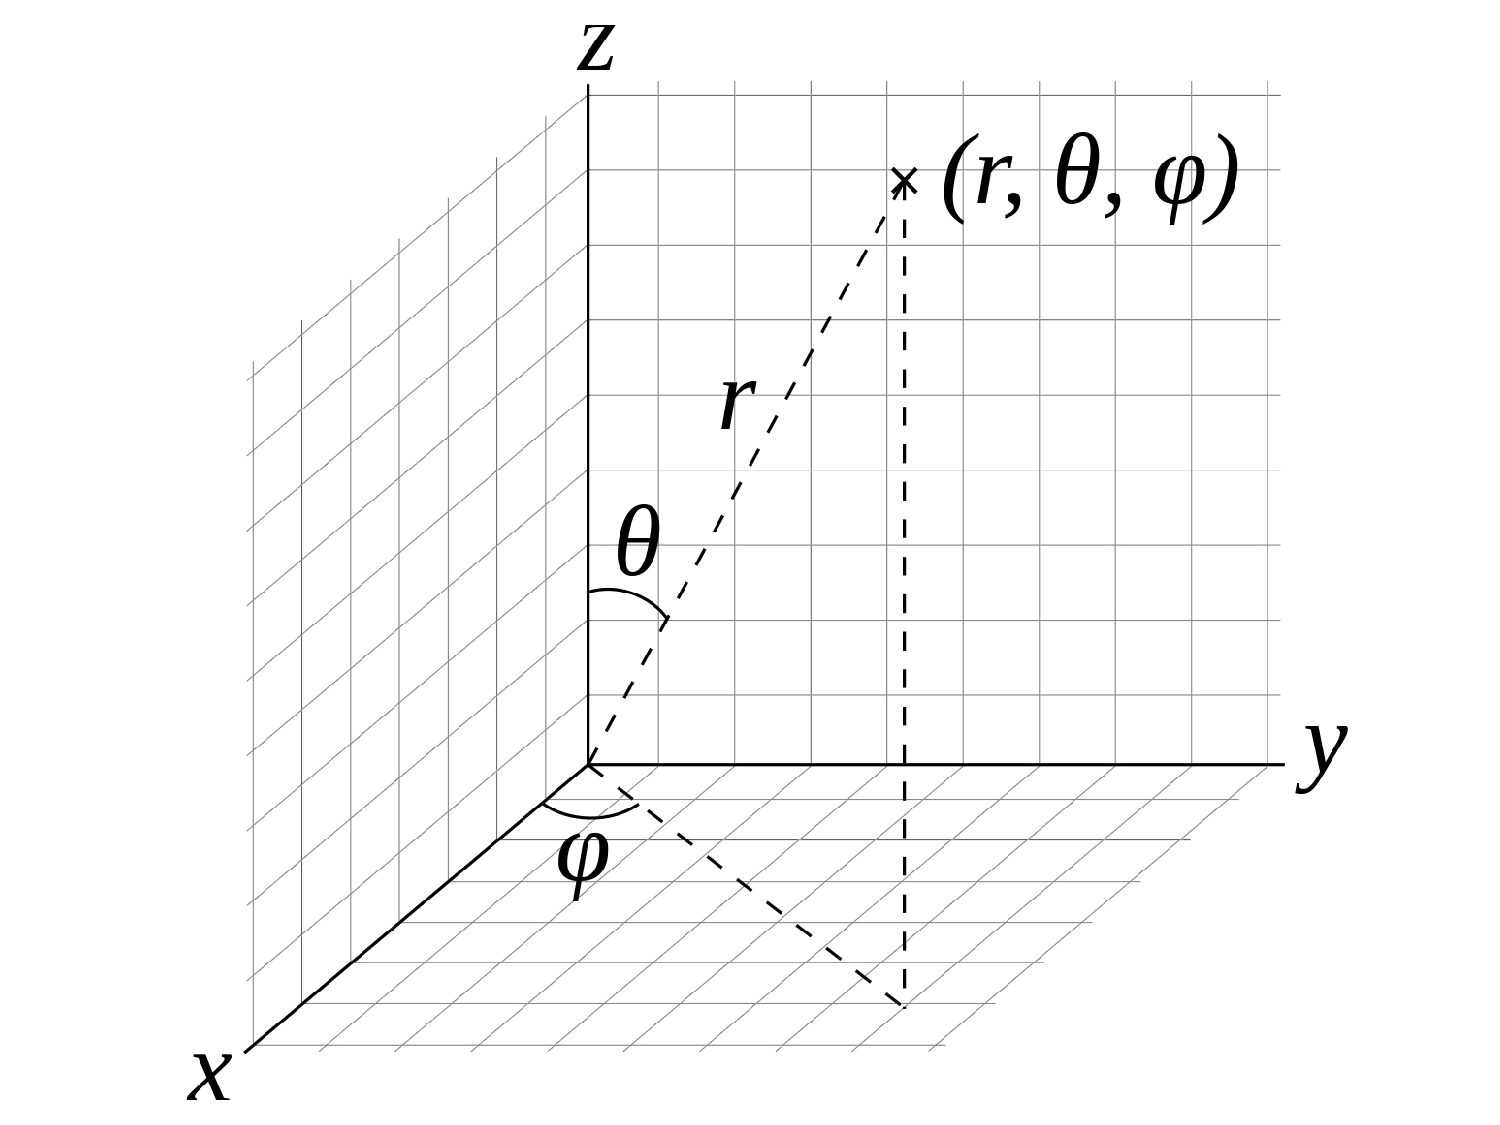
\includegraphics[scale=0.5]{figs/Spherical}
\caption{Graphical demonstration of spherical coordinates.}
\label{fig:hoop}
\end{figure}
\begin{equation}
\begin{cases}
x = r\sin\theta \cos\phi,\\
y = r\sin\theta \sin\phi,\\
z = r\cos\theta.
\end{cases}
\end{equation}
It can be shown that
\begin{equation}
\label{spherical_z_anguar}
\boxed{
L_z = -i\hbar\frac{\partial}{\partial \phi}.
}
\end{equation}
Indeed, $\frac{\partial}{\partial \phi}
=\frac{\partial x}{\partial\phi}\frac{\partial}{\partial x}
+\frac{\partial y}{\partial\phi}\frac{\partial}{\partial y}
+\frac{\partial z}{\partial\phi}\frac{\partial}{\partial z}
= -y\frac{\partial}{\partial x} + x\frac{\partial}{\partial y} 
+ 0
$.

Let's define
\begin{equation}
\Delta_{\phi, \theta}:= \frac{1}{\sin ^2\theta}\cdot\frac{\partial ^2}{\partial \phi ^2}+\frac{1}{\sin \theta}\cdot\frac{\partial }{\partial \theta }\left(\sin \theta \cdot \frac{\partial}{\partial \theta }\right).
\end{equation}
It can be also shown that 
\begin{equation}
\label{spherical_angular}
\boxed{
L^2 = -\hbar \Delta_{\phi, \theta}.
}
\end{equation}
Interestingly, it is well known that:
\begin{equation}
\Delta = \frac{1}{r^2}\Bigg(\Delta _{\phi, \theta}+\frac{\partial }{\partial r}\left(r^2 \cdot\frac{\partial}{\partial r}\right)\Bigg).
\end{equation}
From (\ref{spherical_z_anguar}) and (\ref{spherical_angular}) it is apparent that $[L^2,L_z]=0$. Thus $L_z$ and $L^2$ can be measured simultaneously.

Let's recall associated Legendre polynomials:
\begin{equation}
P_{l,m}(x):=\frac{(-1)^m}{2^l l!} \left(1-x^2\right)^{m/2} \frac{\partial ^{l+m}\left(x^2-1\right)^l}{\partial x^{l+m}}
\end{equation}
for $l=0, 1, \dots$ and $m=-l,\dots, l$.
Now we can define
\begin{equation}
Y_{l,m}(\theta ,\phi )\text{:=}\sqrt{\frac{(2 l+1) (l-m)!}{4 \pi  (l+m)!}} \exp (i m \phi ) P_{l,m}(\cos (\theta )).
\end{equation}
They are eigenvectors of both $L^2$ and $L_z$ with the eigenvalues as in equations below.
\begin{equation}
\boxed{
\begin{cases}
L_z Y_{l,m} = m\hbar Y_{l,m},\\
L^2 Y_{l,m} = l(l+1)\hbar^2 Y_{l,m}\\
\end{cases}
}
\end{equation}
for $l=0, 1, \dots$ and $m=-l,\dots, l$.
\subsection{Motivation for potential operator}

We will assume that potential observable $V$ measures
potential $V(x)$ (we overload $V$ symbol here) in a space point $x$ as an eigenvalue of a Dirac delta at point $x$ (i.e. $\delta_x(z):=\delta(x - z$)).
\begin{equation}
V\delta_x = V(x)\delta_x.
\end{equation}
Let's calculate $V(\psi)$.
\begin{equation}
(V\psi)(x) = \int \delta_x(z) (V\psi)(z)dz = \int (V\delta_x)(z)\psi(z)dz = \int V(z)\cdot \delta_x(z)\psi(z)dz = V(x)\cdot \psi. 
\end{equation}

Second transformation above holds because $V$ is self-adjoint.

\subsection{Proton-electron system}
Let's consider a system of two particles, one with negative elementary charge $-e$ and mass $m_e$ and the other with positive elementary $e$ and mass $m_p$.

To investigate probability amplitude of the relative position of the two particles, according to considerations in Subsection \ref{reduced-mass-in-quantum}, we need to get the following hamiltonian:
\begin{equation}
H \psi = \sum_{i=1}^3 \cfrac{P^2_i}{2\mu}\psi + V\cdot\psi, 
\end{equation}
where $\mu$ is a reduced mass, namely $\mu = \cfrac{m_e m_p}{m_e + m_p}$ and $V$ is an potential energy of the system of two charges governed by Coulomb force:
\begin{equation}
V = - \cfrac{e^2}{4\pi\epsilon_0 r}.
\end{equation} 
For completness let's check if $-\cfrac{\partial V}{\partial x}$ gives us Coulomb force. Let's assume $x=[x_1, x_2, x_3]$ is a radial vector of electron and that proton is in the center of our frame of reference. Obvioulsy $r:=(x_1^2 + x_2^2 + x_3^2)^{\frac{1}{2}}$. Now
\begin{equation}
F_i = -\cfrac{\partial V}{\partial x_i} = -\big(-\cfrac{1}{2}\cdot 2x_i \cdot (-\cfrac{e^2}{4\pi\epsilon_0}(x_1^2 + x_2^2 + x_3^2)^{-\frac{3}{2}})\big) = -x_i \cfrac{e^2}{4\pi\epsilon_0 r^3}.
\end{equation}
Thus
\begin{equation}
\vec{F} = \cfrac{e^2}{4\pi\epsilon_0 r^3}x,
\end{equation}
which is exactly Coulomb force.
Let's then put our Hamiltonian in an abreviated form:
\begin{equation}
H = -\cfrac{\hbar^2}{2\mu}\Delta - \cfrac{e^2}{4\pi\epsilon_0 r}.
\end{equation}
There exist eigen vectors $\psi_{n,l,m}$ of $H$ such that
\begin{equation}
\begin{cases}
H\psi_{n,l,m} = -\cfrac{e^4 \mu }{32 \pi ^2 n^2 \epsilon_0^2 \hbar ^2}\psi_{n,l,m},\\
L^2 \psi_{n,l,m} = l(l+1)\hbar^2 \psi_{n,l,m}\\
L_z \psi_{n,l,m} = m\hbar \psi_{n,l,m},
\end{cases}
\end{equation}
for $n=1,2, \dots$, $l=0, 1, 2, \dots$ and $m=-l, \dots, l$.
The value
\begin{equation}
\boxed{
E_n = -\cfrac{e^4 \mu }{32 \pi ^2 n^2 \epsilon_0^2 \hbar ^2}
} 
\end{equation} 
is an energy level of hydrogen for $n=1,2,\dots$.

We will now present energy levels dependent on fine-structure constant. Let's recall
\begin{equation}
\alpha = \cfrac{e^2}{4\pi\epsilon_0\hbar c}
\end{equation}

Thus

\begin{equation}
E_n = - \alpha^2 \cfrac{\mu c^2}{2 n^2} = - \cfrac{\alpha^2}{2} \cfrac{E_\mu}{n^2},
\end{equation}

where $E_\mu$ is energy equivalent to reduced mass of electron.

\section{Perturbation Theory}
\subsection{Fermis's golden rule}
\label{fermi-golden-rule}
Assume we have a Hamiltonian $H$ with eigenstates base $\ket{\alpha}$ with corresponding eigenvalues $E_\alpha$, where $\alpha$ is a certain parametrisation of the base states. 

\begin{equation}
H \ket{\alpha} = E_{\alpha} \ket{\alpha}.
\end{equation}

Moreover, we assume normalisation $\bra{\alpha}\ket{\beta} = \delta(\alpha - \beta)$. It will be useful to use $\omega_{\beta\alpha} \stackrel{def}{=} E_\beta - E_\alpha$.


Let's assume that $\ket{\alpha t}$ satisfies evolution equation

\begin{equation}
i\cfrac{\partial}{\partial t} \ket{\alpha t} = H\ket{\alpha t},
\end{equation}
and that $\ket{\alpha t_0} = \ket{\alpha}$. Thus, we have
\begin{equation}
\ket{\alpha t} = e^{-itE_\alpha} \ket{\alpha}.
\end{equation}

Note that $\ket{\alpha t}$ is a new basis of quantum states space.
\begin{proposition}
\label{timed-unity-decomposition}
\begin{equation}
\int \ket{\alpha t}\bra{\alpha t} d\alpha = 1.
\end{equation}
\end{proposition}
\begin{proof}
\begin{multline*}\\
\int \ket{\alpha t}\bra{\alpha t}\ket{\alpha_0 t} d\alpha = 
\int \ket{\alpha t} e^{it(E_\alpha - E_{\alpha_0})}\bra{\alpha}\ket{\alpha_0} d\alpha\\
= \int \ket{\alpha t} e^{it(E_\alpha - E_{\alpha_0})} \delta(\alpha - \alpha_0) d\alpha = \ket{\alpha_0 t}.\\
\end{multline*}
\end{proof}

Assume we have another Hamiltonian:
\begin{equation}
H' = H + \epsilon W(t).
\end{equation} 

The following abbreviation will be useful:
$$W(t)_{\beta \alpha} = \bra{\beta} W(t) \ket{\alpha}.$$

Take an arbitrary $\ket{\psi(t)}$ which satisfies evolution equation
\begin{equation}
i\cfrac{\partial}{\partial t}\ket{\psi(t)} = (H + \epsilon W(t)) \ket{\psi(t)}.
\end{equation}

Since (\ref{timed-unity-decomposition}), we can expand $\ket{\psi(t)}$ as 
\begin{equation}
\label{evolution-expansion}
\ket{\psi(t)} = \int \bra{\alpha t}\ket{\psi(t)}\ket{\alpha t}d\alpha.
\end{equation}

Let's calculate
\begin{multline*}\\
i\cfrac{\partial}{\partial t} \bra{\alpha t}\ket{\psi(t)} = \{i \bra{\alpha t}\} \ket{\psi(t)} + \bra{\alpha t}\{i \cfrac{\partial}{\partial t} \ket{\psi(t)}\} = 
\\
= - \bra{\alpha t} H \ket{\psi(t)} + \bra{\alpha t} H + \epsilon W(t)\ket{\psi(t)}= \bra{\alpha t} \epsilon W(t) \ket{\psi(t)}.\\
\end{multline*}

And since (\ref{evolution-expansion}), we can write an equation:
\begin{equation}
\label{central-perturbation-equation}
i\cfrac{\partial}{\partial t} \bra{\beta t}\ket{\psi(t)} = \int \bra{\alpha t}\ket{\psi(t)}\bra{\beta t}\epsilon W(t) \ket{\alpha t}d\alpha.
\end{equation}

Let $c_\beta(t) \stackrel{def}{=}  \bra{\beta t}\ket{\psi(t)}$. Then (\ref{central-perturbation-equation}) will take a form:

\begin{equation}
\boxed{
i\cfrac{\partial}{\partial t} c_\beta(t) = \int c_\alpha t\bra{\beta t} \epsilon W(t) \ket{\alpha t}d\alpha
}
\end{equation}

Let's define operator

 
\begin{equation}
\hat{W}(t)\stackrel{def}{=} e^{itH} W(t) e^{-itH}.
\end{equation}

Hence (\ref{central-perturbation-equation}) becomes
\begin{equation}
i\cfrac{\partial}{\partial t} c_\beta(t) = \int c_\alpha(t)\bra{\beta}\epsilon \hat{W}(t) \ket{\alpha}d\alpha.
\end{equation}

Let's define
\begin{equation}
\ket{u(t)} \stackrel{def}{=}  \int c_\alpha (t) \ket{\alpha} d\alpha.
\end{equation}

Note that $\ket{u(t)}$ satisfies evolution equation
\begin{equation}
i\cfrac{\partial}{\partial t} \ket{u(t)} = \epsilon \hat{W}(t) \ket{u(t)},
\end{equation}

and $\ket{u(t_0)} = \ket{\psi(t_0)}$.

Let 
\begin{equation}
U(t_0, t) = \mathcal{T} \exp(-i\epsilon \int_{t_0}^t ds \hat{W}(s)),
\end{equation}

then since (\ref{generic-linear-solution2})
\begin{equation}
\ket{u(t)} = U(t_0, t) \ket{\psi(t_0)}.
\end{equation}

We are assuming a situation in which the quatum system was in a state $\ket{\alpha}$ at time $t_0$. Then it was eveloved by Hamiltonian $H + \epsilon W(t)$ and at a time $t$ part $\epsilon W(t)$ was ``switched off". We are then interested in probability (or density of probability) $P_{\alpha \to \beta}$ that system ``measured" by $H$ will collapse to the state $\ket{\beta}$.

Assume then $\ket{\psi(0)} = \ket{\alpha}$.

Then
\begin{equation}
P_{\alpha \to \beta} = |\bra{\beta}\ket{\psi(t)}|^2 = |\bra{\beta}\ket{u(t)}|^2.
\end{equation}

Note that
\begin{equation}
\bra{\beta}\ket{u(t)} = \bra{\beta} U(t_0, t) \ket{\alpha},
\end{equation}

Hence,
\begin{equation}
P_{\alpha \to \beta} = |\bra{\beta} U(t_0, t) \ket{\alpha}|^2.
\end{equation}

\begin{lemma}
\label{perturbation-aproximations}
\begin{equation}
\bra{\beta} U(t_0, t) \ket{\alpha} = \delta(\beta - \alpha) + \sum_{n=1}^\infty (-i\epsilon)^n \rho^{\beta,\alpha}_n(t),
\end{equation}
where
\begin{align*}
& \rho^{\gamma_n, \gamma_0}_n(t) = \int_{t_0}^t ds_n \int_{t_0}^{s_n} ds_{n - 1}\dots \int_{t_0}^{s_2} ds_1 \int d\gamma_{n-1} \dots \int d\gamma_1 \\
& \prod_{k=1}^n \exp(is_k(E_{\gamma_k} - E_{\gamma_{k - 1}})) W(s_k)_{\gamma_k \gamma_{k - 1}}.
\end{align*}
\end{lemma}
\begin{proof}
By \ref{integral-version-schrodinger} we have
\begin{equation}
U(t_0, t) = 1 - i\epsilon \int_{t_0}^t ds \hat{W}(s) U(t_0, s).
\end{equation}
Thus

\begin{equation}
\bra{\beta} U(t_0, t) \ket{\alpha} = \delta(\beta - \alpha) - i\epsilon\int_{t_0}^t ds \bra{\beta}\hat{W}(s) U(t_0, s)\ket{\alpha},
\end{equation}

and thus

\begin{equation}
\bra{\beta} U(t_0, t) \ket{\alpha} = \delta(\beta - \alpha) - i\epsilon\int_{t_0}^t ds \bra{\beta}\hat{W}(s)\int d\gamma \ket{\gamma}\bra{\gamma} U(t_0, s)\ket{\alpha},
\end{equation}

\begin{equation}
\bra{\beta} U(t_0, t) \ket{\alpha} = \delta(\beta - \alpha) - \int_{t_0}^t ds \int d\gamma e^{is(E_\beta - E_\gamma)} W_{\beta\gamma}(s) \bra{\gamma}U(t_0, s)\ket{\alpha}.
\end{equation}
Let $K_{\beta, \alpha}(t) = \delta(\alpha - \beta) + \sum_{n=1}^\infty (-i\epsilon)^n \rho^{\beta,\alpha}_n(t)$. It is enough to show that $K_{\beta, \alpha}(t)$ satisfy equation :
\begin{equation}
K_{\beta, \alpha}(t) = \delta(\beta - \alpha) - i\epsilon \int_{t_0}^t ds \int d\gamma e^{is(E_\beta - E_\gamma)} W_{\beta\gamma}(s) K_{\gamma, \alpha}(s).
\end{equation} 
Let's do calculations
\begin{multline*}
\\
\int_{t_0}^t ds \int d\gamma e^{is(E_\beta - E_\gamma)} W_{\beta\gamma}(s) K_{\gamma, \alpha}(s) = 
\int_{t_0}^t ds \int d\gamma e^{is(E_\beta - E_\gamma)} W_{\beta\gamma}(s) 
\bigg(\delta(\gamma - \alpha) + \sum_{n=1}^\infty (-i\epsilon)^n \rho^{\gamma,\alpha}_n(s)  \bigg) \\
= \int_{t_0}^t ds e^{is(E_\beta - E_\alpha)} W_{\beta\alpha}(s) + 
\sum_{n=1}^\infty (-i\epsilon)^n \int_{t_0}^t ds \int d\gamma e^{is(E_\beta - E_\gamma)} W_{\beta\gamma}(s) \rho^{\gamma,\alpha}_n(s)\\
=  \int_{t_0}^t ds e^{is(E_\beta - E_\alpha)} W_{\beta\alpha}(s) + \sum_{n=1}^\infty (-i\epsilon)^n \rho^{\beta,\alpha}_{n+1}(s) = \rho_1^{\beta,\alpha}(t) + \sum_{n=1}^\infty (-i\epsilon)^n \rho^{\beta,\alpha}_{n+1}(s).\\
\end{multline*}
Thus
\begin{multline*}\\
\delta(\beta - \alpha) - i\epsilon \int_{t_0}^t ds \int d\gamma e^{is(E_\beta - E_\gamma)} W_{\beta\gamma}(s) K_{\gamma, \alpha}(s) \\
= \delta(\beta - \alpha)-i\epsilon \rho_1^{\beta,\alpha}(t) + \sum_{n=1}^\infty (-i\epsilon)^{n + 1} \rho^{\beta,\alpha}_{n+1}(s) = K_{\beta, \alpha}(t).\\
\end{multline*}

\end{proof}

We will assume that $W(t) = e^{\eepsilon t} W$, where $W$ is constant in time. We will also take $t_0\to -\infty$. 

Let's try get some useful expression of $U(t_0, t)$.
Let
\begin{equation}
S_n(t_0, t) =  (-i)^n \int_{t_0}^t ds_n \hat{W}(s_n) \int_{t_0}^{s_n} ds_{n - 1} \hat{W}(s_{n-1})\dots \int_{t_0}^{s_2} \hat{W}(s_1)ds_1.
\end{equation}

Then, we have
\begin{equation}
U(t_0, t) = 1 + \epsilon^n \sum_{n=1}^\infty S_n (t_0, t).
\end{equation}

Let's calculate $S_n$:
\begin{multline}\\
S_n(-\infty, t) = (-i)^n \int_{-\infty}^t ds_n \int_{-\infty}^{s_n} ds_{n - 1}\dots \int_{-\infty}^{s_2} ds_1\\
e^{is_nH}We^{i(s_{n-1} - s_n)H}W \dots e^{i(s_1 - s_2)H}We^{-is_1H}e^{\eepsilon(s_n + \cdot + s_1)}.
\end{multline}

Let's do substitution of dummy wariables:
\begin{align*}
&t_n = s_n,\\
&t_{n-1} = s_{n-1} - s_n,\\
&\dots\\
&t_1 = s_1 - s_2.
\end{align*} 

and inversly

\begin{align*}
&s_n =t_n,\\
&s_{n-1} = t_n + t_{n-1}\\
&\dots\\
&s_1 = t_n + t_{n-1} + \cdots + t_1.
\end{align*}

Jacobian determinant of this transformation is 1, then we can write
\begin{align*}\\
&S_n(-\infty, t) = (-i)^n \int_{-\infty}^t dt_n \int_{-\infty}^{0} dt_{n - 1}\dots \int_{-\infty}^{0} dt_1\\
&e^{it_nH}We^{it_{n-1}H}W \dots e^{it_1H}We^{-i(t_n + \cdots + t_1)H}e^{\eepsilon(s_n + \cdot + s_1)}.
\end{align*}

Note that
\begin{align*}
&\bra{\beta}S_n (-\infty, t) \ket{\alpha} = (-i)^n \\
& \bra{\beta} \int^t_{-\infty} dt_n e^{n\eepsilon t_{n}} e^{it_n(E_{\beta} - E_{\alpha})} W\\
& \int^0_{-\infty}dt_{n-1} e^{(n - 1)\eepsilon t_{n - 1}}e^{i(H - E_\alpha)} W\\
& \dots \\
&\int^0_{-\infty}dt_{1} e^{\eepsilon t_1}e^{i(H - E_\alpha)} W \ket{\alpha}.
\end{align*} 

Note that,
\begin{equation}
 \int^0_{-\infty} ds e^{k\eepsilon s} e^{is(H - E_{\alpha})} = \cfrac{i}{E_\alpha - H + ik\eepsilon}.
\end{equation} 

Hence,
\begin{equation}
\bra{\beta}S_n (-\infty, t) \ket{\alpha} = \\
\cfrac{e^{-it(\omega_{\alpha\beta} +in\eepsilon)}}{\omega_{\alpha\beta}+in\eepsilon }
\bra{\beta} W \prod_{k = n - 1}^1 (\cfrac{1}{E_\alpha - H + ik\eepsilon}W) \ket{\alpha}.\\
\end{equation}

Note that the above equation is exact. We will now make a replacement $k\eepsilon \to \eepsilon$. For now, we will motivate it that because we can treat $\epsilon$ as a value which disapears in practice with certain power $\epsilon^n$, thus in practice we need to consider only finite number of operators $S_n$. With this assumption in mind, since we will finally consider limit $\eepsilon \to 0$, $k\eepsilon$ is as good as $\eepsilon$. This step leaves us with certain distaste, we will need to make a deeper discussion of it in the future.

Keeping above in mind, let's define the operator
\begin{equation}
\label{transition-operator}
T_{\eepsilon}  \stackrel{def}{=}  \sum_{n = 1}^\infty \epsilon^n W \big(\cfrac{1}{E_\alpha - H + i\eepsilon}W\big)^{n - 1}.
\end{equation}

Let's make now a precise distinction let
\begin{equation}
U(t_0, t) = \mathcal{T} \exp(-i\epsilon \int_{t_0}^t ds e^{isH}W e^{-isH})
\end{equation}

and

\begin{equation}
U_\eepsilon(t_0, t) = \mathcal{T} \exp(-i\epsilon \int_{t_0}^t ds \hat{W}(s)).
\end{equation}

Thus
\begin{equation}
\bra{\beta}U_\eepsilon (-\infty, t) \ket{\alpha} = \delta(\beta - \alpha) + \cfrac{e^{-it(\omega_{\alpha\beta} +i\eepsilon)}}{\omega_{\alpha\beta}+i\eepsilon } \bra{\beta}T_{\eepsilon} \ket{\alpha}.
\end{equation}

Note that
\begin{equation}
S_n (-\infty, 0) \ket{\alpha} =  \big(\cfrac{1}{E_\alpha - H + i\eepsilon}W\big)^n \ket{\alpha},
\end{equation}

and hence
\begin{equation}
U_\eepsilon(-\infty, 0) \ket{\alpha} = \ket{\alpha} + \epsilon^n \sum_{n=1}^\infty \big(\cfrac{1}{E_\alpha - H + i\eepsilon}W\big)^n \ket{\alpha}.
\end{equation}

From the above
\begin{equation}
U_\eepsilon(-\infty, 0) \ket{\alpha} = \ket{\alpha} + \big(\cfrac{1}{E_\alpha - H + i\eepsilon}\epsilon W\big)U(-\infty, 0) \ket{\alpha}.
\end{equation}

Let's define
\begin{equation}
\ket{\psi_\alpha} \stackrel{def}{=} U_\eepsilon(-\infty, 0) \ket{\alpha}.
\end{equation}

Then we have
\begin{equation}
\ket{\psi_\alpha} = \ket{\alpha} + \big(\cfrac{1}{E_\alpha - H + i\eepsilon}\epsilon W\big)\ket{\psi_\alpha}.
\end{equation}

This is called Lippman-Schwinger equation.

By \ref{transition-operator}, we have
\begin{equation}
T_{\eepsilon}\ket{\alpha} = \epsilon W \ket{\psi_\alpha}. 
\end{equation}

For the rest of argumentation we will assume that we will operate on states $\ket{\phi}$ for which there exists self-adjoint $T$ such that 
$T_{\eepsilon}\ket{\phi} - T\ket{\phi} = O(\eepsilon)\ket{\phi}$, 
where $O(\eepsilon)$ is some polynomial error operator.

We will try to calculate $\cfrac{d}{dt} P_{\alpha\to\beta}$. We have
\begin{equation}
P_{\alpha\to\beta} = \bra{\beta}U (-\infty, t) \ket{\alpha}\bra{\beta}U (-\infty, t) \ket{\alpha}^*.
\end{equation}

Let's prepare
\begin{equation}
\bra{\beta}U_\eepsilon (-\infty, t) \ket{\alpha} = \delta(\beta - \alpha) + \cfrac{e^{\eepsilon t}e^{-it\omega_{\alpha\beta}}}{\omega_{\alpha\beta}+i\eepsilon } \bra{\beta}T_\epsilon \ket{\alpha}.
\end{equation}

\begin{equation}
\cfrac{d}{dt}
\bra{\beta}U_\eepsilon (-\infty, t) \ket{\alpha} = -ie^{\eepsilon t}e^{-it\omega_{\alpha\beta}}\bra{\beta}T_\eepsilon \ket{\alpha}.
\end{equation}

Then
\begin{align*}
&\cfrac{d}{dt} \big( \bra{\beta}U_\eepsilon(-\infty, t) \ket{\alpha}\bra{\beta}U_\eepsilon(-\infty, t) \ket{\alpha}^*\big) = \\
& \bigg(\delta(\beta - \alpha) + \cfrac{e^{\eepsilon t}e^{-it\omega_{\alpha\beta}}}{\omega_{\alpha\beta}+i\eepsilon } \bra{\beta}T_\eepsilon \ket{\alpha}\bigg)ie^{\eepsilon t}e^{it\omega_{\alpha\beta}}\bra{\alpha}T^{\dagger}_\eepsilon \ket{\beta} + \\
& \bigg(\delta(\beta - \alpha) + \cfrac{e^{\eepsilon t}e^{it\omega_{\alpha\beta}}}{\omega_{\alpha\beta}-i\eepsilon } \bra{\alpha}T^{\dagger}_\eepsilon \ket{\beta}\bigg)(-i)e^{\eepsilon t} e^{-it\omega_{\alpha\beta}}\bra{\beta}T_\eepsilon \ket{\alpha} = \\
& - \delta(\alpha - \beta) e^{\eepsilon t}\sin(t\omega_{\alpha\beta}) + ie^{\eepsilon t}\big(\cfrac{1}{\omega_{\alpha\beta}+i\eepsilon} - \cfrac{1}{\omega_{\alpha\beta}-i\eepsilon}\big)\bra{\alpha}T^{\dagger}_\eepsilon \ket{\beta} \bra{\beta}T_\eepsilon \ket{\alpha} = \\
& \delta(\alpha - \beta) e^{\eepsilon t}\sin(t\omega_{\beta\alpha})
+ i e^{\eepsilon t} \cfrac{-i2\eepsilon}{\omega_{\beta\alpha}^2 + \eepsilon^2} \bra{\alpha}T^{\dagger}_\eepsilon \ket{\beta} \bra{\beta}T_\eepsilon \ket{\alpha} \to_{\eepsilon\to 0}\\
&\delta(\alpha - \beta) \sin(t\omega_{\beta\alpha}) + 2\pi\delta(\omega_{\beta\alpha})
|\bra{\beta}T\ket{\alpha}|^2.
\end{align*}

Thus
\begin{equation}
\cfrac{d}{dt} P_{\alpha\to\beta} = \delta(\alpha - \beta) \sin(t\omega_{\beta\alpha}) + 2\pi\delta(\omega_{\beta\alpha})
|\bra{\beta}T\ket{\alpha}|^2.
\end{equation}

To simplify equations lets assume $T_{\beta\alpha} \stackrel{def}{=} \bra{\beta}T\ket{\alpha}$.

Let $\Omega$ will be some set of base states ``accesible'' from state $\ket{\alpha}$.

\begin{equation}
\cfrac{d}{dt} P_{\alpha\to{\Omega}} 
= 2\pi \int_{\Omega} d\beta \, \delta(E_\beta - E_\alpha)
T_{\beta\alpha}^2.
\end{equation}

Because we know that $\ket{\beta}$ are eigenstates of $H$, we can find other parametrisation $\beta \mapsto E, \gamma$, where $E = E_\beta$. In such parametrisation, we have

\begin{align*}
& \cfrac{d}{dt} P_{\alpha\to{\Omega}} 
= 2\pi \int_\Omega dE d\gamma \, \delta(E - E_\alpha) T_{\beta(E, \gamma)\alpha}^2 \bigg|\frac{\partial \beta}{\partial E \partial \gamma}\bigg| = \\
& 2 \pi \int_{\Omega(E_{\alpha})} d\gamma\,  T_{\beta(E_\alpha, \gamma)\alpha}^2 \bigg| \frac{\partial \beta}{\partial E \partial \gamma}\bigg|_{E = E_\alpha}.
\end{align*}

The derived equation is called Fermi Golden Rule.
\begin{equation}
\boxed{
\cfrac{d}{dt} P_{\alpha\to{\Omega}} 
= \frac{2 \pi}{\hbar} \int_{\Omega(E_{\alpha})} d\gamma\,  T_{\beta(E_\alpha, \gamma)\alpha}^2 \bigg| \frac{\partial \beta}{\partial E \partial \gamma}\bigg|_{E = E_\alpha}
}
\end{equation}  

In case $\ket{\beta}$ are not degenerated on $\Omega$ (i.e. $E_\beta \not= E_\beta'$ for $\beta \not=\beta'$), we have $E \mapsto \beta$, where $E = E_\beta$.

\begin{equation}
\boxed{
\cfrac{d}{dt} P_{\alpha\to\beta(E_\alpha)} 
= \cfrac{2 \pi}{\hbar} T_{\beta(E_\alpha)\alpha}^2 \bigg| \frac{\partial \beta}{\partial E}\bigg|_{E = E_\alpha}
}
\end{equation}  

\subsection{Stationary Perturbation}
Let's assume our hamiltonian has a form
\begin{equation}
H = H_0 + \epsilon W,
\end{equation}
where complete set of eignestates and eigenvalues of unperturbed hamiltonian $H_0$ is known
\begin{equation}
H_0 \psi^0_n = E^0_n \psi^0_n.
\end{equation}
We assume also that energy levels are not degenerated, i.e.
$E_i \not= E_j$ for $i\not=j$.
The goal of perturbation theory is to determine solutions of 
\begin{equation}
H\psi = E \psi,
\end{equation}
as
\begin{equation}
E = E_k = \sum_{n} E^{(n)}_k\epsilon^n
\end{equation} 
\begin{equation}
\psi = \psi_k = \sum_{m}a_{m,k} \psi_m^0, 
\end{equation}
where 
\begin{equation}
a_{m,k} = \sum_{n=0}^\infty a^{(n)}_{m,k} \epsilon^n. 
\end{equation}
It can be proven (e.g. \cite{walter-greiner2001}[11.1]) that
\begin{equation}
\begin{cases}
E_k^{(0)} = E^0_k, \\
E_k^{(1)} = \mel{\psi_k^0}{W}{\psi_k^0},\\
E_k^{(2)} = \sum_{n\not=k} \cfrac{|\mel{\psi_n^0}{W}{\psi_k^0}|^2}{E^0_n - E^0_k},\\
\dots
\end{cases}
\end{equation}
and
\begin{equation}
\begin{cases}
a^{(0)}_{m, k} = \delta_{m,k},\\
\dots
\end{cases}
\end{equation}
\subsection{Degeneracy}
Assume that for a given level of energy $E^0_n$ in unperturbed hamiltonian $H_0$, we have a series of eigenfunctions $\psi^0_{n,\beta}$ where $\beta=1,2, ..., f_n$. Such level is called $f_n$-fold degenerate.

Solutions $E_{n,\beta}^{(1)}$ of the below equation (\ref{degeneracy-matrix-split}) with unknown variable $E^{(1)}_n$ determin the split of energy level $E^0_n$ into levels $E_{n,\beta} \approx E_n^0 + \epsilon E^{(1)}_{n,\beta} $ in perturbed Hamiltonian $H_0 + \epsilon W$. 

\begin{equation}
\label{degeneracy-matrix-split}
\det\begin{bmatrix}
    \mel{\psi^0_{n,1}}{W}{\psi^0_{n,1}} - E_n^{(1)} & \mel{\psi^0_{n,1}}{W}{\psi^0_{n,2}} & \dots  & \mel{\psi^0_{n,1}}{W}{\psi^0_{n,f_n}}\\
    \mel{\psi^0_{n,2}}{W}{\psi^0_{n,1}} &  \mel{\psi^0_{n,2}}{W}{\psi^0_{n,2}} - E_n^{(1)} & \dots  & \mel{\psi^0_{n,2}}{W}{\psi^0_{n,f_n}} \\
    \vdots & \vdots & \ddots & \vdots \\
    \mel{\psi^0_{n,f_n}}{W}{\psi^0_{n,1}} & \mel{\psi^0_{n,f_n}}{W}{\psi^0_{n,2}} & \dots  & \mel{\psi^0_{n,f_n}}{W}{\psi^0_{n,f_n}} - E_n^{(1)}
\end{bmatrix} = 0.
\end{equation}
The above is proven in (e.g. \cite{walter-greiner2001}[11.2]). To get above equation from matrix equation there, one needs to notice that $E^0 - E = -\epsilon E^{(1)}$ and then remove factor $\epsilon$ from the matrix. The equation in form similiar to (\ref{degeneracy-matrix-split}) is also in \cite{desai2010}[16.4 Degenerate States].
\subsection{Time-Dependent Perturbation}
We assume that the hamiltonian is given by
\begin{equation}
H = H_0 + W(t)
\end{equation}
We assume that $W(t)$ is a small perturbation and acts only in time interval $[0, T]$.
Let $\psi^0_n$ be stationary solutions of
\begin{equation}
H_0 \psi^0_n = E_n \psi^0_n.
\end{equation}
Time evolution is given by
\begin{equation}
\psi^0_n(t) = e^{-\frac{i}{\hbar}E_n t}\psi^0_n.
\end{equation}
We will be interested in an evolution
\begin{equation}
\label{time-dependent-perturbation-evolution}
i\hbar\cfrac{\partial \psi_n(t)}{\partial t} = H\psi_n(t),
\end{equation}
where
\begin{equation}
\psi_n(0) = \psi^0_n.
\end{equation}
Next we will be intrested in the probability for the transition from state $\psi_n(t)$ to $\psi^0_m$ in the period $[0,T]$.
We assume that we start in the state $\psi_n(0) = \psi^0_n$, then the state evolve under the perturbed hamiltonian $H$ according to equation $\ref{time-dependent-perturbation-evolution}$. At the time $t=T$ perturbation $W$ is ``turned off'' and we measure the energy of the state. We want to know the probability that our final state will be $\psi^0_m$, which is expressed by
\begin{equation}
|\braket{\psi^0_m}{\psi_n(t)}|^2.
\end{equation}
Let's express $\psi_n(t)$ in basis $\psi^0_k(t)$:
\begin{equation}
\psi_n(t) = \sum_k a_{n,k}(t) \psi^0_k(t).
\end{equation}
Note that
\begin{equation}
|\braket{\psi^0_m}{\psi_n(t)}|^2 = |a_{n,m}(t)|^2.
\end{equation}
Coefficients $a_{n,m}$ are given by the following system of differential equations
\begin{equation}
i\hbar \cfrac{d a_{n,m}(t)}{dt} = \sum_{k} a_{n,k}(t) \mel{\psi^0_m}{W(t)}{ \psi^0_k} e^{i\omega_{mk}t},
\end{equation}   
where
\begin{equation}
\omega_{mk} = \cfrac{E_m - E_k}{\hbar}.
\end{equation}
The first order aproximation of $a_{n,m}(t)$ is
\begin{equation}
a_{n,m}(t) \approx a^{(1)}_{n,m} = \delta_{nm} - \cfrac{i}{\hbar}\int_0^t \mel{\psi^0_m}{W(\tau)}{ \psi^0_n} e^{i\omega_{mn}\tau}d\tau.
\end{equation}
The above is proven in (e.g. \cite{walter-greiner2001}[11.4]).
\end{document}